%% ----------------------------------------------------------------
%% Article.tex
%% ---------------------------------------------------------------- 

%% You mostly won't have to worry about this file

\documentclass{ecsarticle}     % Use the Article Style
%\documentclass{IEEEtran}
\graphicspath{{../Figures/}}   % Location of your graphics files
\usepackage{natbib}            % Use Natbib style for the refs.
\usepackage{lipsum}
\removecolourlinks    % Uncomment this command to remove colour from any links
%\input{Definitions}            % Include your abbreviations
%% ----------------------------------------------------------------


\begin{document}
\frontmatter
\title      {ELEC6089 High Voltage Insulation Systems Assignment 1}
\authors    {\texorpdfstring{\href{mailto:tjs1g10@ecs.soton.ac.uk}{Thomas J. Smith}}{Thomas J. Smith}, 
\texorpdfstring{\href{mailto:dm4g10@ecs.soton.ac.uk}{David Mahmoodi}}{David Mahmoodi},
\texorpdfstring{\href{mailto:bh8g10@ecs.soton.ac.uk}{Brendan Hickman}}{Brendan Hickman}, 
\texorpdfstring{\href{mailto:pplf1g10@ecs.soton.ac.uk}{Patrick P. L. Fong}}{Patrick P. L. Fong}}
%\department  {Electronics and Computer Science}
\group       {HV AC 275kV Bushing Design}
%\addresses  {\groupname\\\deptname\\\univname}
\addresses  {\univname}
\date       {\today}
\subject    {}
\keywords   {}
\maketitle
\begin{abstract}
The advantages to work in high voltages come with drawbacks, one of the major drawbacks is the increase in complexity of required insulation system associated with voltage level. In high voltage transformer, bushings are required to avoid various electrical breakdown mechanisms caused by the potential difference from high potential equipments to the surrounding earth objects i.e. potential difference between the high voltage conducting cable and the transformer casing. This report starts by discussing the different types of breakdown in high voltage systems and the stress control methods used in relatively lower voltages and DC systems. High voltage AC solutions are discussed, derivation of capacitive stress control in bushing designs and simulated to illustrate the effects of the the two capacitive stress control methods. 
\end{abstract}
%\tableofcontents
%\listoffigures
%\listoftables

%% -----------------------
%% lstpatch.sty
%% -----------------------
%% lstpatch cannot be distributed with these files. I believe it is only needed if the
%% \lstlistoflistings is used. So this has been turned off by default. Re-add if required:
%% \usepackage{lstpatch}
%% \lstlistoflistings
%% You will need to download lstpatch, possibly from:
%% http://web.mit.edu/texsrc/source/latex/listings/lstpatch.sty
%% -----------------------



%\listofsymbols{ll}{$w$ & The weight vector}
\mainmatter
\section{Introduction}
%A brief review on field design in HV equipment.
The design of electrical equipment always involves an aspect of insulation design.
For the safe and efficient operation of electrical equipment it is necessary to have an electrical circuit and a means of isolating this circuit from the surrounding environment \cite{warne2005newnes}.
Power systems contain a complex structure of generators, transmission lines, transformers, switchgear and more. 
All of these different devices require an appropriately selected insulation material in order to isolate the mechanical casings and support structures from the high voltage components \cite{james2008condition}.

The purpose of this report is to describe the design and simulation of a high voltage bushing. Bushings are an integral part of power system insulation. 
IEEE standard C57.19.00 describes a bushing as ``an insulating structure, including a through conductor or providing a central passage for such a conductor, with provision for mounting on a barrier, conducting or otherwise, for the purpose of insulating the conductor from the barrier and conducting current from one side of the barrier to the other.''\cite{1440990}.
Bushings are required for situations such as connecting the external conductor to the internal windings of a transformer through the walls of the metal oil tank.
The walls of the transformer housing will be grounded, but need to be shielded from the incoming high voltage conductor, hence the use of a bushing \cite{warne2005newnes}.
An example of this usage can be seen in figure \ref{Figure:BothBushPics}, as 400kV grid conductors enter an oil filled transformer casing.
The shedding on the outer cylinder can be seen in figure \ref{Figure:BothBushPics} which helps increase electrical strength in wet conditions \cite{warne2005newnes}.

\begin{figure}[!htb]
  \centering
  \subfigure[Transformer wall connection]{
    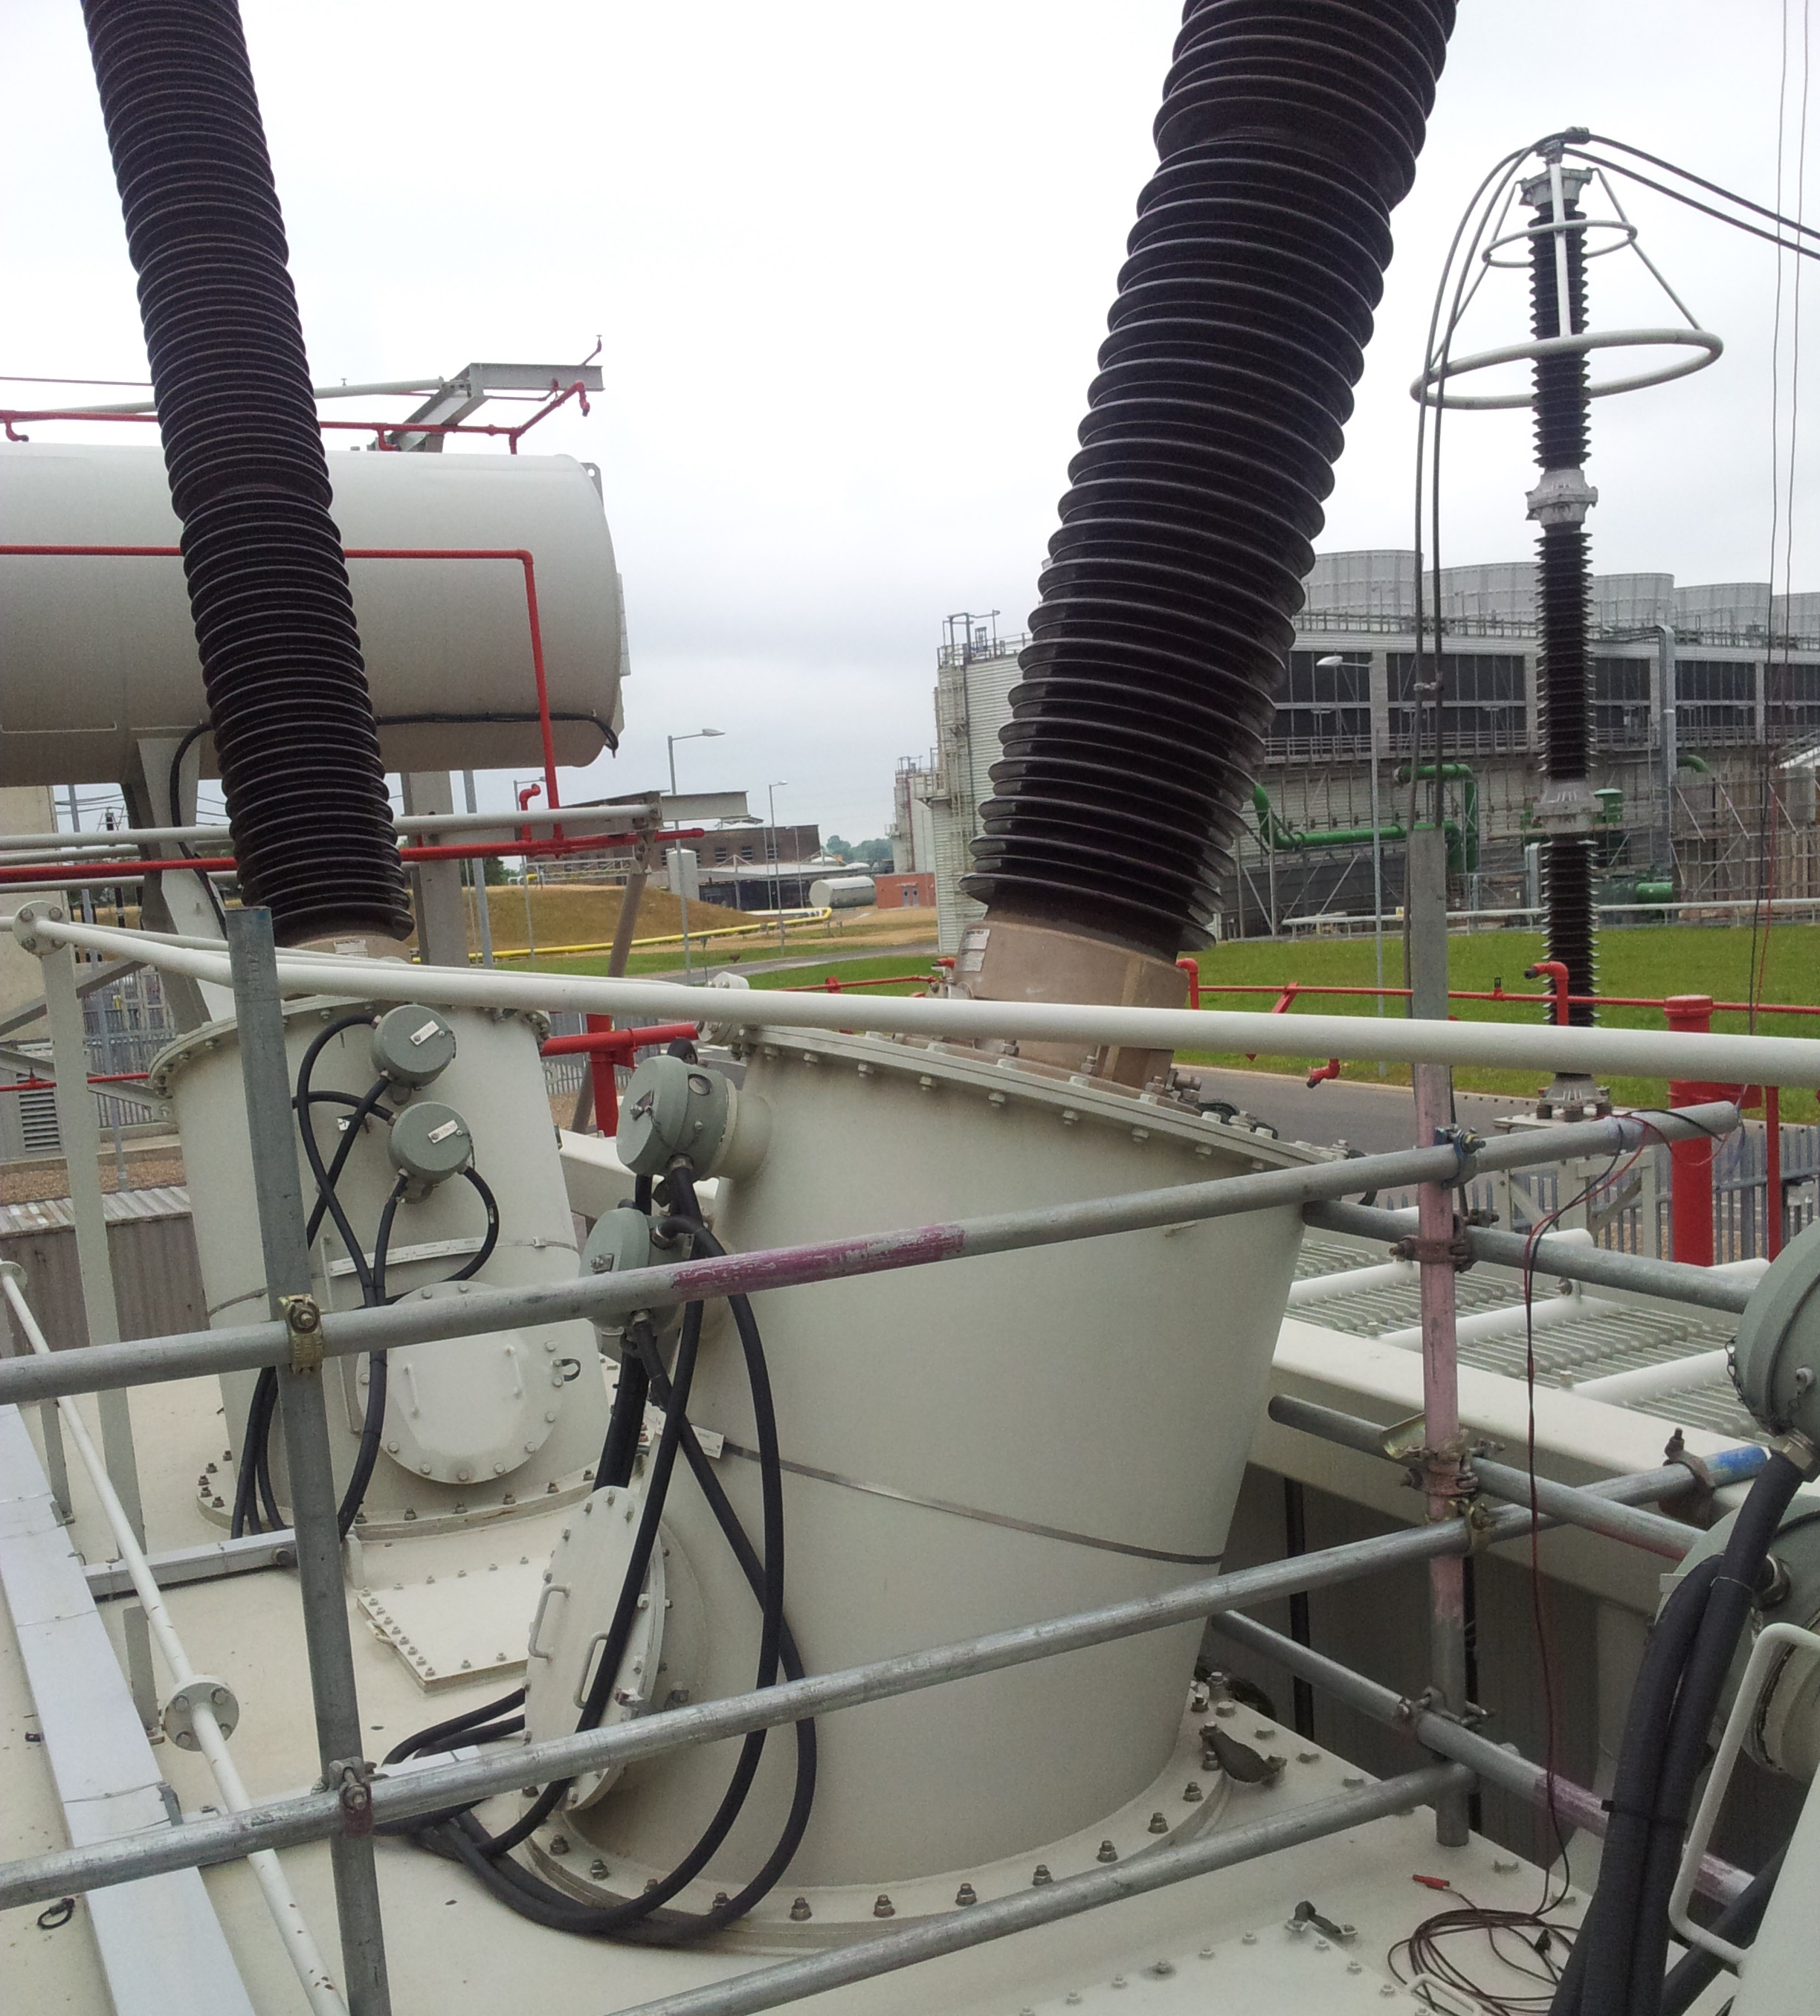
\includegraphics[height = 6cm]{StaythorpeHVBushing.jpg} 
	\label{Figure:Bush1}
  }
  \subfigure[Wide view]{
    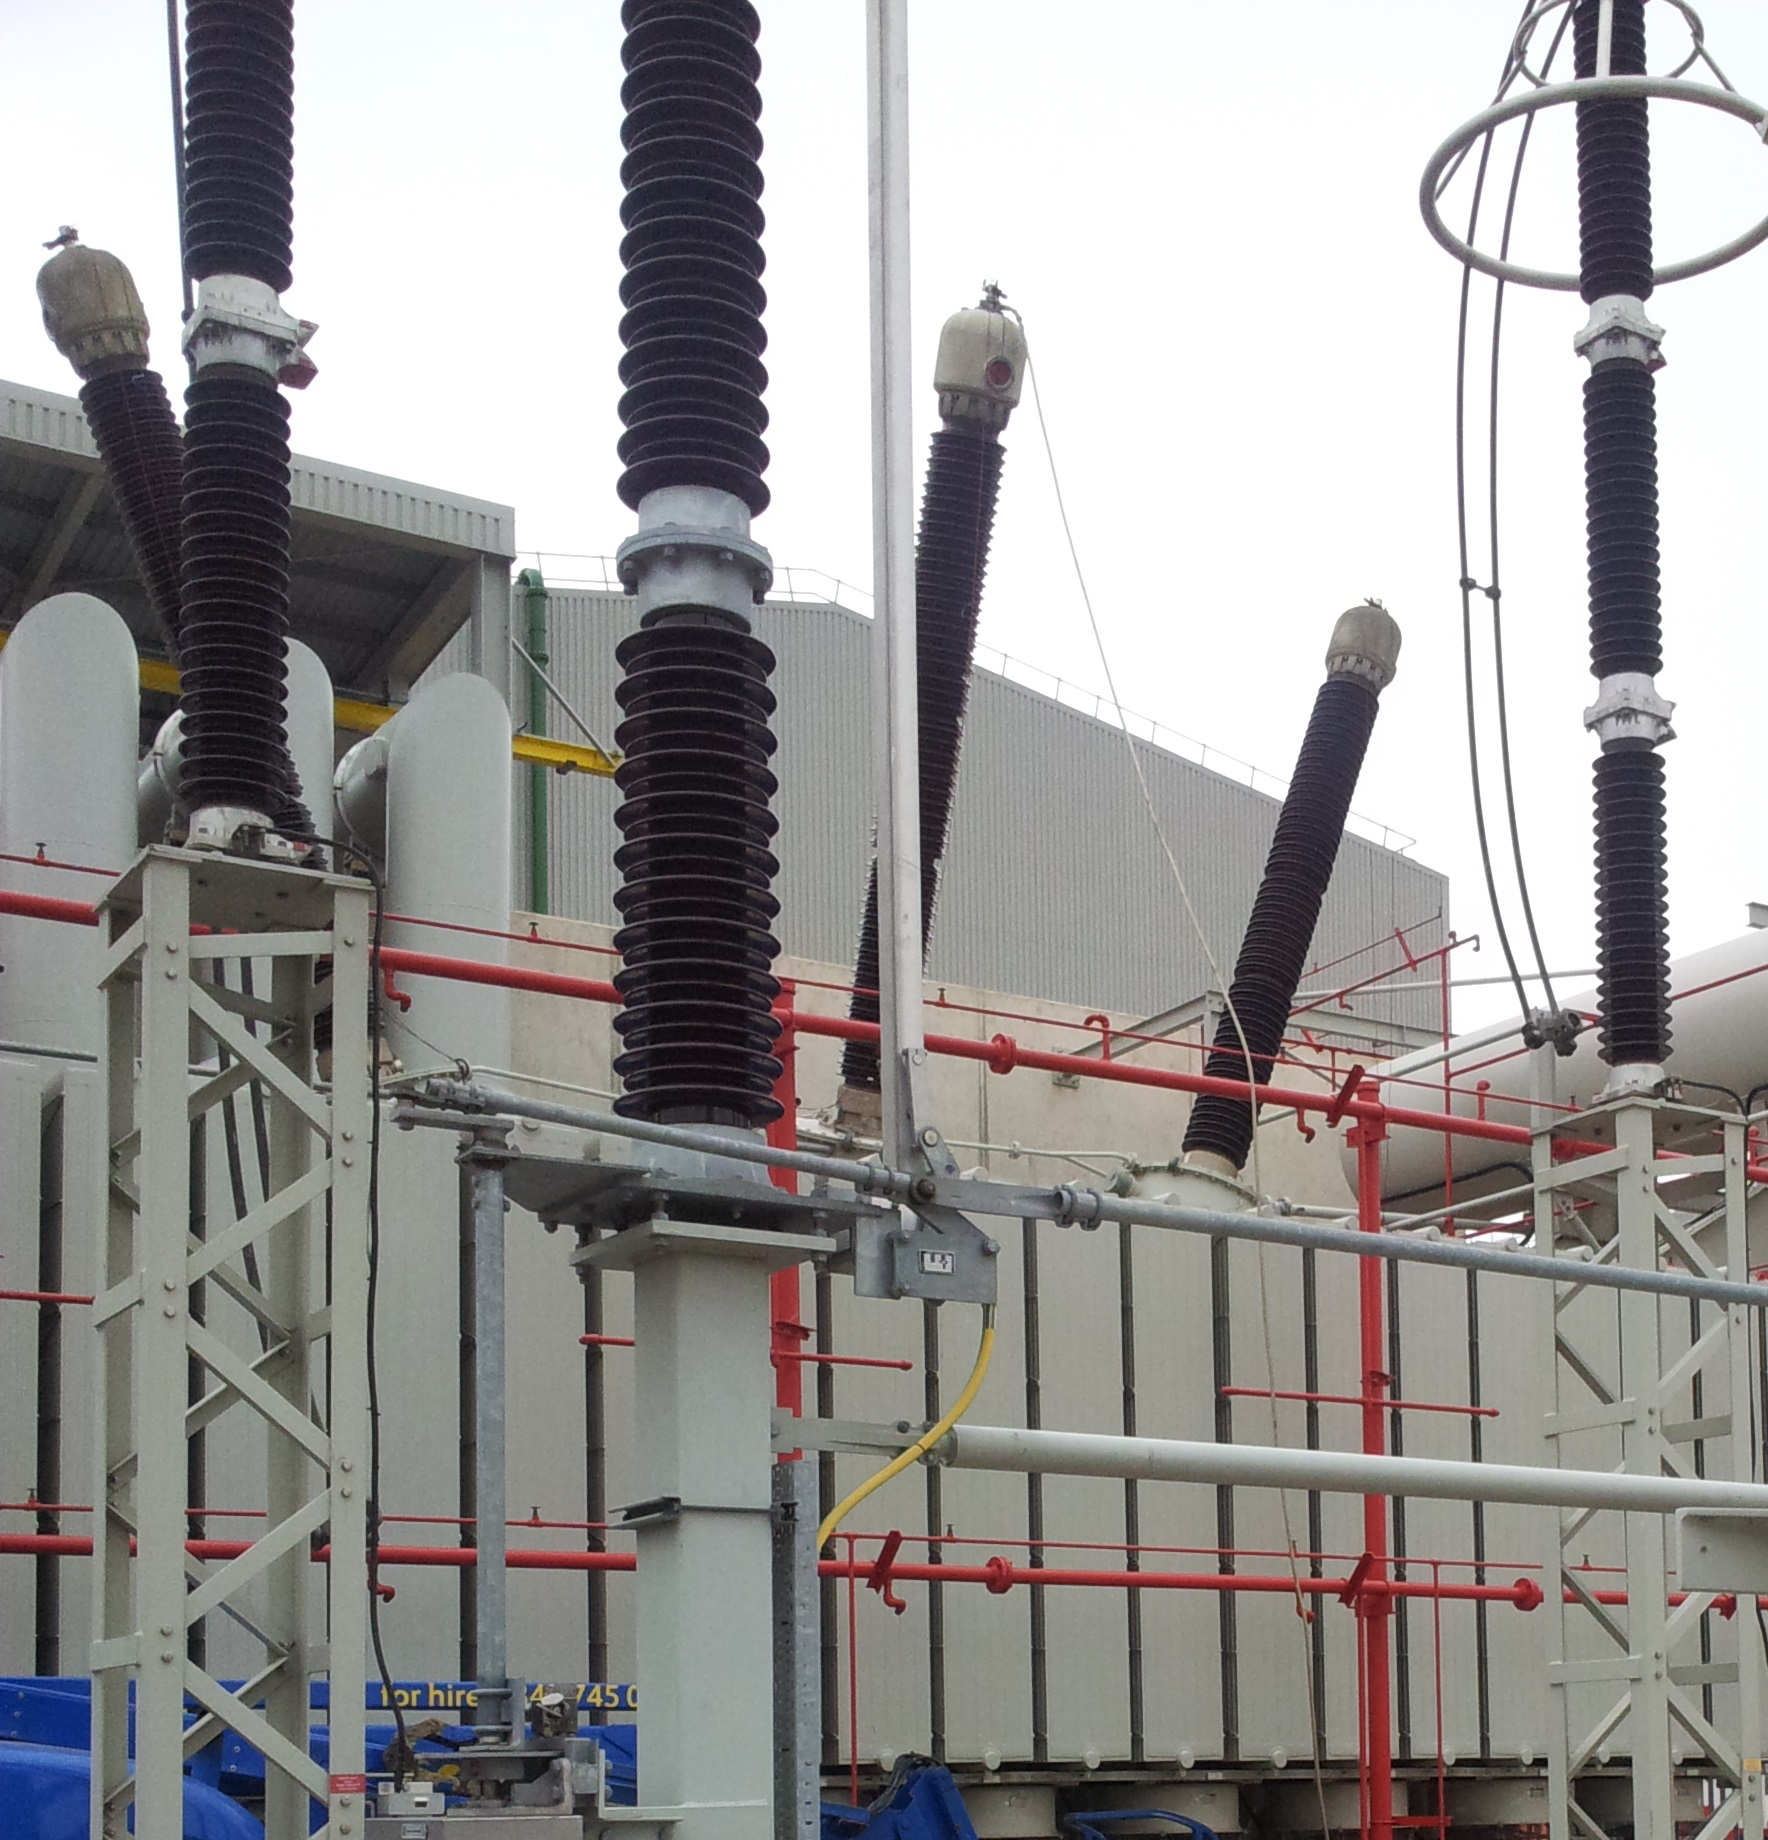
\includegraphics[height = 6cm]{StaythorpeHVBushingWide.jpg} 
	\label{Figure:Bush2}
  }
\caption{High Voltage Bushings on the 400kV Transformers at Staythorpe CCGT Power Station, Newark, UK (Taken by TJS)}
  \label{Figure:BothBushPics}
\end{figure}


% !TeX spellcheck = en_GB
% !TeX root = ReportMain.tex
\section{Overview of Grading Methods} \label{s:method}
Electric field stress control is important in the design of many power system elements, especially cable terminations and bushings \cite{james2008condition}.
Failure of a bushing can damage the power transformer it is protecting, which can be an expensive mistake \cite{warne2005newnes}.
Bushings are required to withstand Electrical, Mechanical and Thermal stresses as defined in the IEEE standard C57.19.00 \cite{1440990}.
The design of the bushing is largely determined by the insulation material chosen and the resolution of these conflicting sources of stress.
A good bushing design has insulation that can withstand the applied voltage and thermal characteristics appropriate for the current carried by the conductor \cite{harlow2004electric}.

\begin{figure}[!h]
   \centering
   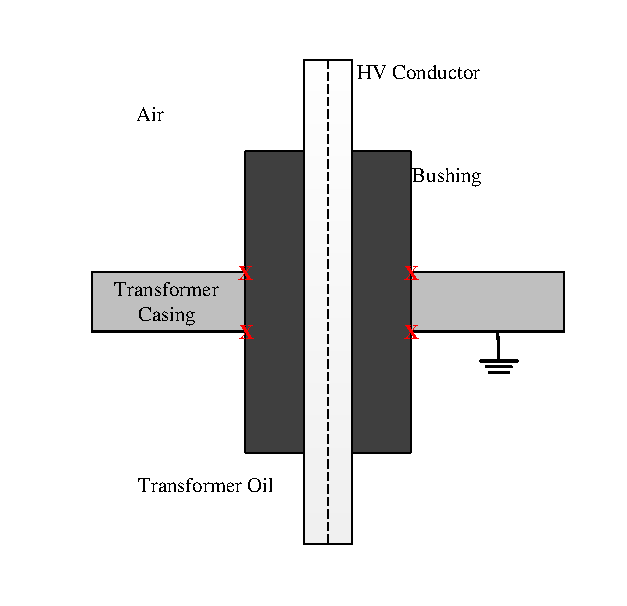
\includegraphics[width = 0.5\textwidth]{GenericBushing.pdf}
   \caption{The Bushing Problem}
   \label{figure:problem}
\end{figure}

The problem grading methods attempt to resolve is laid out in figure \ref{figure:problem}.
The grounded transformer casing is shown in light grey which is perpendicular to the the bushing insulation shown in dark grey and the high voltage conductor in white.
The top of the bushing is exposed to air, while the other side is exposed to transformer oil.
Conducting a numerical analysis or simulation would show that the conductor surface within the plane of the transformer casing and at the points marked by red crosses would experience high electric field stress.
The bushing insulation is designed to withstand the high electric field between the conductor and the transformer casing, however at the points marked with crosses the interface between the solid insulation and the air/transformer oil would cause surface discharge leading to relatively low flashover voltages \cite{kuffel2000high}.
It is therefore necessary to develop methods of reducing electric field stress to a more uniform distribution for both functional purposes and the economic use of space and materials \cite{james2008condition}.

\subsection{Low Voltage and DC Solutions}
There are several methods that can be used dependent upon the application.
Low voltage solutions include internal and external screening electrodes, while resistive stress control can be used for DC applications. Sometimes these solutions are used in combination to achieve an acceptable result.

%%starts here(PPLF)

\subsubsection{External Screening Electrode}

External screening electrodes are parts outside the conductor that are not electrically connected to the conductor. 
They are made of metal conductors such as aluminium. 
Corona ring designs are intended to reduce the electric field strength around the bushing terminal, hence reducing the chance of corona or partial discharge.
Grading ring designs are intended to reduce the potential gradient of insulator, hence reducing the chance of electrical breakdown. 
These screening electrodes come with various shapes according to the different designs. 
The main types of design take the shape of sphere, toroid or ring. 
These are shapes which prevent regions of intense electric field strength by varying the electric potential distribution and help contain electric field as much as possible. 
The reduction in corona discharge not only reduces the power loss, it also suppresses the ageing speed of the insulator. 
An example of these can be seen on figure \ref{Figure:Bush1} and figure \ref{Figure:Bush2}, where they are placed at the top of the bushings. 
The diameters of these designs are closely related to the electric field strength around the electrode, so the diameters of these designs must be carefully considered in order to avoid electrical breakdown.

\subsubsection{Internal Screening Electrode}

Internal screening electrodes are also used to control the electric potential distribution so the electric field strength is within acceptable level to avoid chance of breakdown. They are placed inside the insulator and usually in a pressurised gas. Some existing designs have the shape of internal electrode in a 3D cone like shape and maybe referred as a deflector and there are also designs which are disk shape. An example of the field distribution with the cone shape deflector inserted is demonstrated in figure \ref{figure:deflector}.

\begin{figure}[!h]
   \centering
   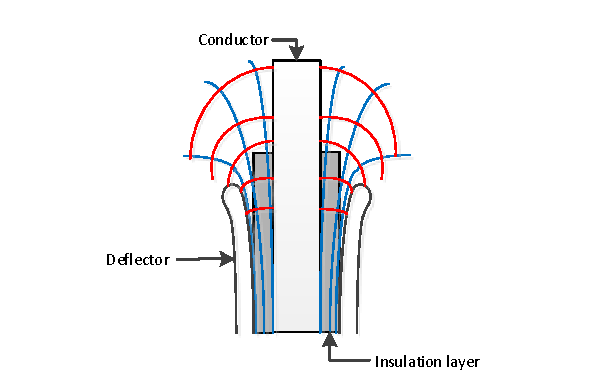
\includegraphics[width = 0.7\textwidth]{Deflector.pdf}
   \caption{Field distribution with deflector}
   \label{figure:deflector}
\end{figure}

\subsection{Capacitive Grading} \label{ss:CapacitiveGrading}
Capacitive grading was first proposed by R.Nagel of Siemens in a German paper published in 1906 \cite{harlow2004electric}.
The value of this type of arrangement was quickly recognised, and is now industry standard practice for AC bushing designs for 25kV - 1500kV applications \cite{james2008condition}.
The general concept of the design is illustrated in figure \ref{figure:fieldgeneric}, showing the isolated foils inserted inside the solid bushing insulation.
Shown in red in figure \ref{figure:fieldgeneric} is the potential field with no grading, and in blue with the isolated conductive foils inserted.
It shows that the whole dielectric is much more evenly stressed with the capacitive grading method.
\begin{figure}[!h]
   \centering
   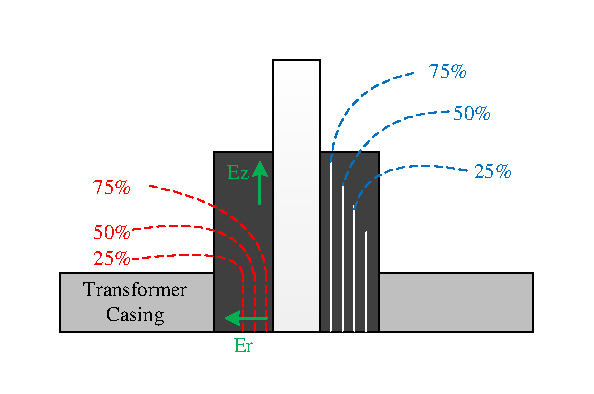
\includegraphics[width = 0.7\textwidth]{BushingFieldDiagram.pdf}
   \caption{Field Distribution both without capacitive grading (shown in red) and with capacitive grading (shown in blue), modified from \cite{james2008condition}}
   \label{figure:fieldgeneric}
\end{figure}

The insulation is stressed in both a radial and axial direction, which sum to give the tangential field.
The radial component $E_r$ can cause breakdown of the insulating material, while the axial component $E_z$ can cause surface discharge along the boundary \cite{Ahmed11}.
Attention must be paid to the design and shape of the boundary, so that the critical value for inception voltage for surface discharge is not exceeded \cite{david2}.
These can be seen in green in figure \ref{figure:fieldgeneric}.
These sum up to give the tangential field $E_t$.

Before proceeding, it is first necessary to introduce some terms.
\begin{figure}[!h]
   \centering
   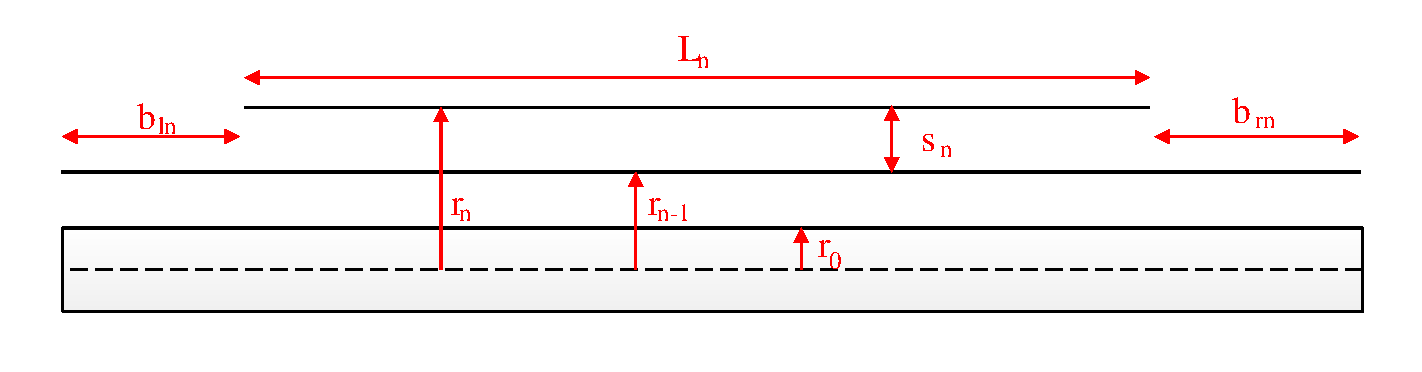
\includegraphics[width = \textwidth]{GradingSymbols.pdf}
   \caption{Symbols for calculating capacitive grading, modified from \cite{Ahmed11}}
   \label{figure:terms}
\end{figure}
Firstly, the radius of the foil is referenced from the centre of the conductor, and termed $r_n$. 
The spacing between each foil is defined in equation \ref{eq:Spacing}.
\begin{equation}
   \label{eq:Spacing}
   S_n = r_n - r_{n-1}
\end{equation}
Additionally, the length of each foil is referred to as $L_n$ and the difference in length on the right and left side between each foil is termed $b_{ln}$ and $b_{rn}$. 
Symmetric double sided capacitive grading is achieved when $b_{ln}=b_{rn}$ \cite{Ahmed11}. 
The total number of foils in the system is $N$.
Also note that subscript $n$ denotes the outermost foil.

Inserting isolated conducting foils forms a set of coaxial capacitor units \cite{kuffel2000high}.
The equation for the capacitance of one of these capacitors depends on the radial displacement $r_n$ and length of each foil $L_n$, as in equation \ref{eq:Cn}.
\begin{equation}
   \label{eq:Cn}
   C_n =\displaystyle\displaystyle\frac{2\pi\epsilon L_{n}}{ln(\displaystyle\frac{r_{n}}{r_{n-1}})}
\end{equation}

The most widely used method to choose the dimensions and locations of the foils is double sided capacitive grading, of which there are two variants; radial grading and axial grading \cite{Ahmed11}.
The aim of capacitive grading is to evenly distribute the electric field between the foils.
To achieve this, an even voltage difference between foils is required as in equation \ref{eq:voltagediff}, where $V$ is the total voltage difference between the conductor and the casing, $N$ is the number of foils required and $\Delta V$ is the voltage between each foil \cite{David1}.
\begin{equation}
   \label{eq:voltagediff}
   \Delta V = \displaystyle\frac{V}{N}
\end{equation}

For the voltage between each foil to be constant, as in equation \ref{eq:voltagediff}, the capacitance between each consecutive pair of foils must also be constant. This is expressed as $C_n = C_{n-1} = \dots = C_0$

\subsubsection{Radial Grading} \label{Section:RadialGrading}
The radial spacing and dimension of each foil is determined in the following derivation, which has been verified and modified from \cite{kuffel2000high}.
In radial grading, the radial component of the electric field $E_r$ is kept constant between all the foils.
The radial electric field is related to the voltage difference and the spacing between each foil, as in equation \ref{eq:radialfield}. $\Delta V$ is already defined as a constant from equation \ref{eq:voltagediff}, and so to have equal field the foil spacing $S_n$ should also be constant. 
\begin{equation}
   \label{eq:radialfield}
   E_r = \displaystyle\displaystyle\frac{\Delta V}{S_n} = Constant
\end{equation}

Given this condition and equation \ref{eq:Cn} for coaxial capacitance, the length of each foil is required to change from foil to foil.
The lengths and radii of consecutive foils can be calculated from the relationship in equation \ref{eq:expcaps}.
%Taking the condition described previous that $C_n = C_{n-1} = \dots = C_0$ and equation \ref{eq:Cn}, equation \ref{eq:expcaps} can be written.
\begin{equation}
   \label{eq:expcaps}
   C_n = \displaystyle\frac{2\pi\epsilon L_{n}}{ln(\displaystyle\frac{r_{n}}{r_{n-1}})} = C_{n-1} = \displaystyle\frac{2\pi\epsilon L_{n-1}}{ln(\displaystyle\frac{r_{n-1}}{r_{n-2}})} = \dots = C_{1} = \displaystyle\frac{2\pi\epsilon L_{1}}{ln(\displaystyle\frac{r_{1}}{r_{0}})}
\end{equation}

The common factor of $2\pi\epsilon$ cancels from equation \ref{eq:expcaps} giving a simple equation linking the lengths and radial displacements of consecutive foils, as in equation \ref{eq:expcaps2}.
\begin{equation}
   \label{eq:expcaps2}
   \displaystyle\frac{L_{n}}{ln(\displaystyle\frac{r_{n}}{r_{n-1}})} = \displaystyle\frac{ L_{n-1}}{ln(\displaystyle\frac{r_{n-1}}{r_{n-2}})} = \dots = \displaystyle\frac{ L_{1}}{ln(\displaystyle\frac{r_{1}}{r_{0}})}
\end{equation}

An approximate solution for thin foils can then be found.
Under the thin foil assumption, $r_{n} = r_{n-1} + S_n$ and $\displaystyle\frac{S_n}{r_n}<<1$ even for the smallest radii of the inner foil.
This is shown in equation \ref{eq:simplefoils}.
%Equation \ref{eq:simplify} allows the simplification of equation \ref{eq:expcaps2} to equation \ref{eq:simplefoils}.

\begin{equation}
   \label{eq:simplify}
   ln(\displaystyle\frac{r_n}{r_{n-1}}) = ln\displaystyle\frac{1}{1-(\displaystyle\frac{S_n}{r_n})} \approx \displaystyle\frac{S_n}{r_n}
\end{equation}

\begin{equation}
   \label{eq:simplefoils}
   L_{n}r_{n} \approx L_{n-1}r_{n-1} \approx \dots \approx L_{1}r_{1}
\end{equation}

Equation \ref{eq:expcaps2} can then be used to determine an exact solution while equation \ref{eq:simplefoils} can be used to find an approximate solution in conjunction with initial data regarding the length and radial displacement of the first foil and the spacing of the foils to calculate the parameters of all the other foils in the bushing. Nevertheless, it should be noted, at this stage, that $r_0$ refers to the surface of the conductor.

\subsubsection{Axial Grading}
In axial grading, the axial component of the electric field $E_z$ is kept constant between all of the foils. 
The following equations prove that the length of each foil must decay by a constant value for each consecutive foil, and the radius at which it is placed is determined by a simple iterative formula.

The axial electric field is related to the voltage difference and the length change between each consecutive foil as in equation \ref{eq:axialfield}. 
Under symmetric capacitive grading, $b_n = b_{ln} = b_{rn}$ with reference to figure \ref{figure:terms}. 
$\Delta V$ is already defined as a constant from equation \ref{eq:voltagediff}, and so to have equal field, the change in foil length $b_n$ should also be constant.
\begin{equation}
   \label{eq:axialfield}
   E_z = \displaystyle\frac{\Delta V}{b_n} = Constant
\end{equation}

The relationship between $L_n$ and $b_n$ is defined in figure \ref{figure:terms}, as explained in equation \ref{eq:length}.
\begin{equation}
   \label{eq:length}
   L_n = L_{n-1} - 2b_n
\end{equation}

Since equation \ref{eq:axialfield} requires the change in foil length $b_n$ to be constant, equation \ref{eq:Cn} for coaxial capacitance requires the radius of each foil to change from foil to foil.
This can be simplified to a similar form as equation \ref{eq:expcaps2}, except that the initial information required, in this case, are different. The necessary parameters are: the length of the first foil($L_1$), the radius of conductor and first foil($r_0,r_1$). However, for initial calculation of $L_n (n=1,2,...N)$ the size of the constant difference in length between each of the foils should be known.All other lengths and radii can then be calculated.

In case of axial grading where different material is used on each side of the bushing ($b_{ln} \neq b_{rn}$) similar calculation is carried out for each side. The total length of each foil is found  by adding $L_{ln}$ and $L_{rn}$. Furthermore, position of each foil could be calculated using the recursive formulae at equation \ref{eq:Axial} 

\begin{equation}
   \label{eq:Axial}
   \displaystyle r_n= \displaystyle  r_{(n-1)} \displaystyle \exp\big( \displaystyle  \frac{L_n}{L_{1}}ln(\displaystyle \frac{r_1}{r_0})\big)
\end{equation}


%\inote{here}

%
%When a conductor is surrounded by concentric foils of dielectric constant $\epsilon$ that is much greater than $\epsilon_{0}$, the system can be treated as a set of coaxial cylindrical capacitor units connected in series.
%In this derivation, the simplest boundary condition is assumed, that is the mean value of the radial field $E_r$ remains constant within the foils.
%The foils are assumed to be of equal thickness, denoted by $\delta$.
%Each of the foils forms a coaxial capacitor stressed by the equal voltage $\Delta V = E_{r}\delta$ providing all capacitances are equal.
%The capacitance of each foil is equal providing $C_n = C_{n-1} = C_0$ where equation \ref{eq:Cn} gives the value of each capacitance.


%This can be expanded as in equation \ref{eq:lengthequals}.
%\begin{equation}
%   \label{eq:lengthequals}
%   \displaystyle\frac{L_n}{ln(\displaystyle\frac{r_{n-1}}{r_{n}})} = \displaystyle\frac{L_{n-1}}{ln(\displaystyle\frac{r_{n-2}}{r_{n-1}})} = \displaystyle\frac{L_1}{ln(\displaystyle\frac{r_{0}}{r_{1}})}
%\end{equation}



%The two methods for solving the recursive equation in equation \ref{eq:simplefoils} is through either radial or axial grading \cite{Ahmed11}.
%In radial grading, the spacing of the foils $S_n$ is assumed to be constant. 
%This means the length of the foils decreases as it it approaches the outer foils of the bushing.
%Equation \ref{eq:evenspace} gives the method to calculate $S_n$ which can then be used in the recursive equation \ref{eq:recursive}, which is a simple form of equation \ref{eq:simplefoils}.
%\begin{equation}
%   \label{eq:evenspace}
%  S_n = \displaystyle\frac{Outer Diameter - Conductor Diameter}{N-1}
%\end{equation}
%
%\begin{equation}
%   \label{eq:recursive}
%  L_{n+1}= L_{n}\displaystyle\frac{r_{n}}{r_{n} + S_{n}}
%\end{equation}


%Radial grading better suits the purposes of this paper, since there is no requirement to assume the length of the final foil.

%\inote{TS - We could derive the recursive equation for axial grading given an assumption of the final foil length here.}
\section{Capacitive Grading Techniques}
HV bushing and two capacitive grading methods.

\lipsum
\section{Design Details}
The reference model for this project is shown in figure \ref{figure:refproblem}. 
The reference design is a paper impregnated with oil bushing with 21 aluminium foils of $100\mu m$.
One side of the bushing is exposed to air, the other to oil, similar to a transformer bushing.
The diameter of the conductor is 100mm, the bushing diameter is 300mm.
The length of the first foil is 5000mm long, and fixed 2mm into the bushing at the conductor voltage.
The outer foil is also set 2mm inside the bushing and is directly connected to the earthed flange.
The conductor is used at 275kV AC voltage, and the design is known to be flawed.
\begin{figure}[!h]
   \centering
   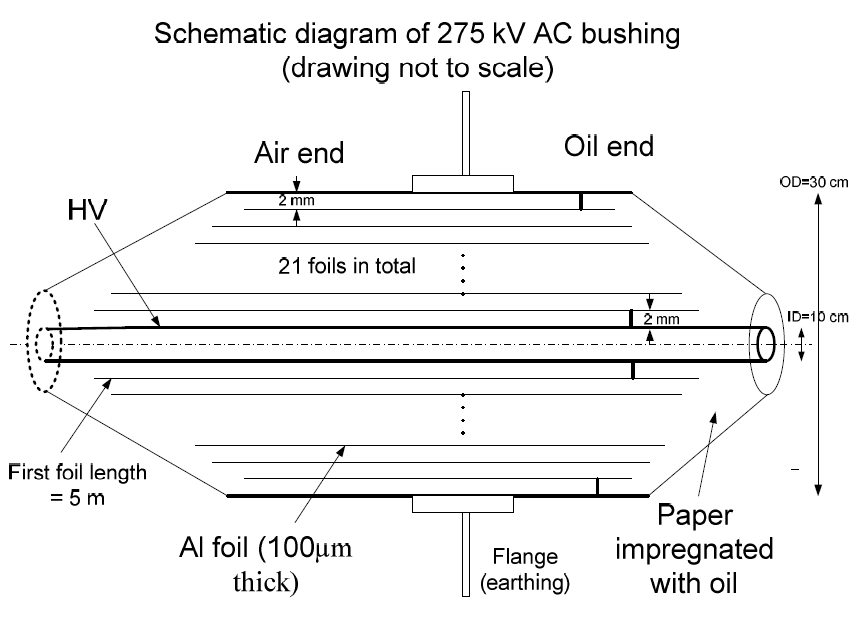
\includegraphics[width = 0.7\textwidth]{ReferenceDiagram.png}
   \caption{The reference problem taken from \cite{Chen14}}
   \label{figure:refproblem}
\end{figure}

A Matlab script was developed to take a required number of foils, and the inner and outer dimensions of the bushing, to calculate the radial location and length of each foil using the radial grading method as described in section \ref{ss:CapacitiveGrading}.
This script was built to be easily customisable for any number of foils and any initial values, to cater for the calculation of improved designs.
It automatically outputs data in a form for direct input into the COMSOL model, and auto-updates a \LaTeX  file containing the data in table \ref{table:radialvals21}.
Finally, the script plots the calculated foil positions in a crude graph shown in figure \ref{Figure:Both21plots}.
Particularly in figure \ref{Figure:21plot2} the decay shape can be observed as expected.
This allows a quick verification of the scripts accuracy before proceeding to simulation.

\begin{table}[!htb]
\caption{Radial Grading Calculations Results}
\label{table:radialvals21}
\begin{center}
\begin{tabular}{cc}
\toprule
\textbf{Radius(mm)} & \textbf{Length(mm)} \\ \toprule
52.00 & 5000.00 \\ 
56.80 & 4577.46 \\ 
61.60 & 4220.78 \\ 
66.40 & 3915.66 \\ 
71.20 & 3651.69 \\ 
76.00 & 3421.05 \\ 
80.80 & 3217.82 \\ 
85.60 & 3037.38 \\ 
90.40 & 2876.11 \\ 
95.20 & 2731.09 \\ 
100.00 & 2600.00 \\ 
104.80 & 2480.92 \\ 
109.60 & 2372.26 \\ 
114.40 & 2272.73 \\ 
119.20 & 2181.21 \\ 
124.00 & 2096.77 \\ 
128.80 & 2018.63 \\ 
133.60 & 1946.11 \\ 
138.40 & 1878.61 \\ 
143.20 & 1815.64 \\ 
148.00 & 1756.76 \\ 
\bottomrule
\end{tabular}
\end{center}
\end{table}


\begin{figure}[!htb]
  \centering
  \subfigure[Wide View]{
    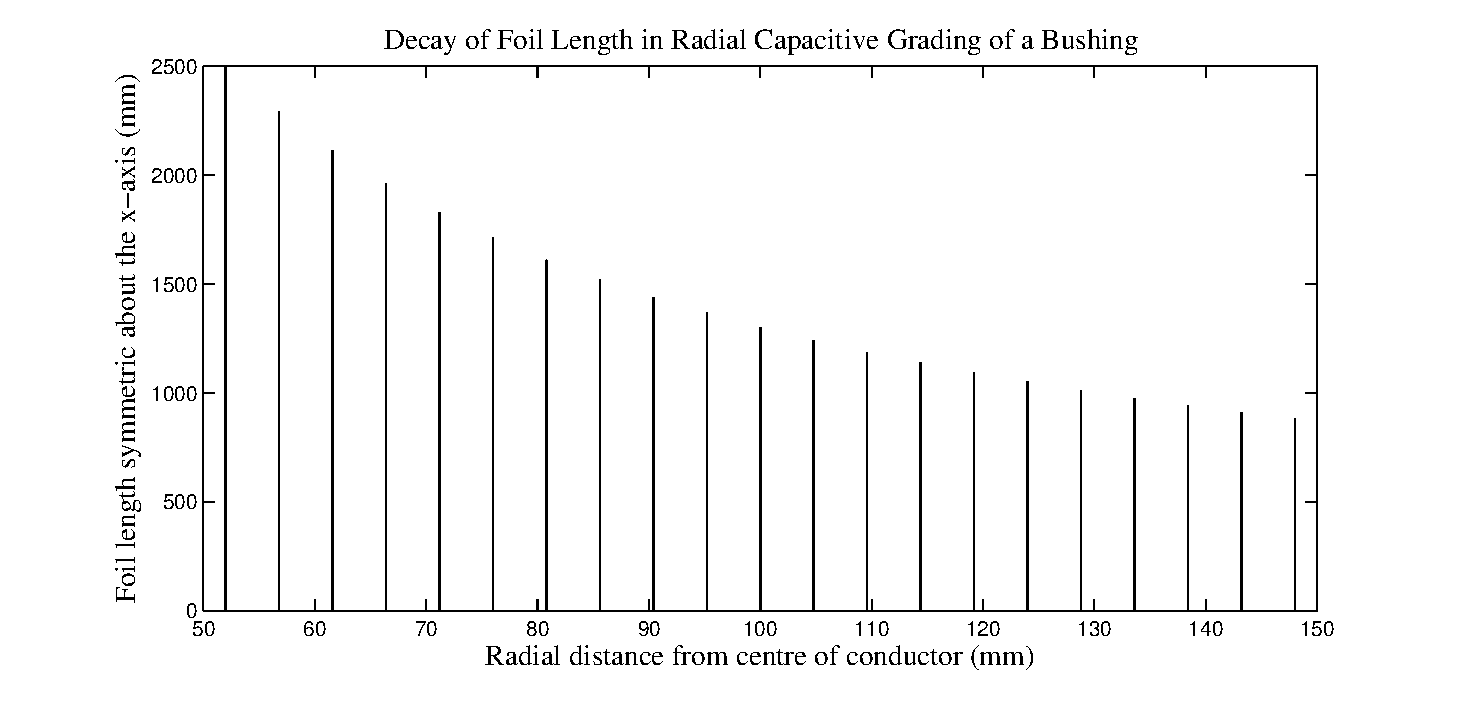
\includegraphics[height = 6cm]{../Matlab_Calculations/RadialGrade21ProfileWide.eps} 
	\label{Figure:21plot1}
  }
  \subfigure[Real Perspective]{
    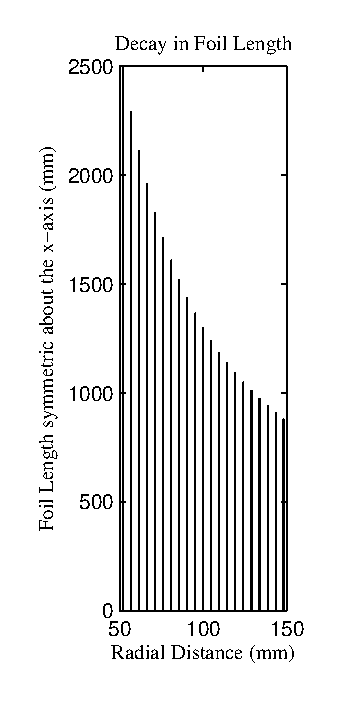
\includegraphics[height = 6cm]{../Matlab_Calculations/RadialGrade21ProfileSquash.eps} 
	\label{Figure:21plot2}
  }
\caption{Representation of foil radial position and length}
  \label{Figure:Both21plots}
\end{figure}

The final information required to be able to proceed to the simulation phase is the relative permittivity of each material.
This was gathered from \cite{Ahmed11} and is shown in table \ref{table:perm}.

\begin{table}[!htb]
\caption{Relative Permittivity of Materials}
\label{table:perm}
\begin{center}
\begin{tabular}{cc}
\toprule
\textbf{Material} & \textbf{Relative Permittivity ($\epsilon_r$)} \\ \toprule
Air & $1$ \\
Oil &$ 2.2$ \\
Paper Impregnated with Oil &$ 4$ \\
Aluminium & $10^8$\\
\bottomrule
\end{tabular}
\end{center}
\end{table}


%  Field_Modelling.tex
% !TeX spellcheck = en_GB
% !TeX root = ReportMain.tex

\section{Modelling Results}
The following simulations were completed using the COMSOL multiphysics software package.
COMSOL is a professional finite element simulation package able to model a variety of physical features.
The following models are created using the AC/DC module, which is used to simulate electric and magnetic fields \cite{ComsolACDC}.
Specifically, the electrostatics interface is used. 
This solves a charge conservation equation for a given voltage and spacial distribution of charge \cite{ComsolACDC}.

\subsection{Finite Element Methods (FEM)}
There are inherent difficulties in solving the partial differential equations that govern many practical engineering problems \cite{kuffel2000high}.
Despite knowing the equations and appropriate boundary conditions that govern a problem, many are complicated by irregular geometries or other discontinuities.
Numerical methods allow approximate solutions to be obtained for problems intractable by analytic methods \cite{meshkatoddini2006study}.
In an analytic solution, the whole system is governed by a mathematical equation valid for the entire region of interest. 
Although these differential equations are often mathematically compact, it is difficult to obtain an answer unless the system is unreasonably simplified \cite{meshkatoddini2006study}.
In FEMs, the complex geometry is broken into a series of much smaller and simpler geometries \cite{kuffel2000high}.
These geometries can be squares, rectangles or triangles in 2D or the 3D equivalent shapes. 
These simpler shapes form interconnected subregions for which an approximate function, usually a high order polynomial, can be used to represent the actual function.
If the complex is split into an adequate number of simple shapes, these approximate functions closely matches the exact solution \cite{meshkatoddini2006study}.

By default COMSOL uses a triangular discretisation to split up a complex geometry in a process called meshing.
This forms an unstructured grid of triangles, allowing the mapping of complex or curved geometries.
Other numerical methods such as Finite Difference Methods require a structured grid, hence FEMs are more flexible with regards to geometry \cite{kuffel2000high}.
Meshing requires an initial understanding of the expected outcomes of the problem, so that the mesh can be refined in areas of interest.
Each triangular element is approximated by a linear interpolation of the potential at the vertices of the triangle.
A set of linear algebraic equations are formed by minimising the error between the actual solution and a set of approximate linear trial functions \cite{meshkatoddini2006study}.

\subsection{Equation Derivation and Boundary Conditions}
The electrostatics interface of the AC/DC COMSOL module uses the electric potential $V$ to calculate static electric fields.
A Poisson type partial differential equation is derived using classical electrostatics and Gauss' Law \cite{hayt2012engineering}.

By taking Gauss's Law:
\begin{equation}
\nabla.\mathbf{D} = \rho v
\end{equation}
the equation for electric flux density $\mathbf{D}$:
\begin{equation}
\mathbf{D} = \epsilon_0\epsilon_r\mathbf{E}
\end{equation}
this can be combined with the equation for a static electric field:
\begin{equation}
\mathbf{E} = -\nabla V
\end{equation}
to give by substitution:
\begin{equation}
\nabla.\mathbf{D} = \nabla.(\epsilon_0 \epsilon_r \mathbf{E}) = -\nabla.(\epsilon_0 \epsilon_r \nabla V) = \rho v
\end{equation}
which is more usually written:
\begin{equation}
\nabla^{2}V = -\frac{\rho v}{\epsilon_0 \epsilon_r}
\end{equation}
where $\epsilon_0$ is the permittivity of free space, $\epsilon_r$ is the relative permittivity of the material, $\mathbf{E}$ is the electric field strength and $\rho v$ is the volume charge density.

In the special case where there is zero volume charge density, that is $\rho v = 0$ then the equation simplifies to Laplace's Equation:
\begin{equation}
\nabla^{2}V = 0
\end{equation}

The models used in this paper are 2D axisymmetric, meaning that a 2D model is used to describe a 3D object that can be rotated $360^o$ about a central point $r=0$ to give a 3D geometry.
This assumes that not only is the geometry the same in the $\varphi$ direction, but also that the electric potential is constant.
In this case, Poissons equation can be rewritten in cylindrical coordinates for a 2D axisymmetric model, it is multiplied by r to ensure there are no singularities at $r=0$ \cite{meshkatoddini2006study}.
\begin{equation}
\begin{bmatrix} 
\frac{\partial}{\partial r} \\
\frac{\partial}{\partial z}
\end{bmatrix}^T
.(r \begin{bmatrix}
\frac{\partial V}{\partial r} \\
\frac{\partial V}{\partial z}
\end{bmatrix})
= -\frac{r\rho v}{\epsilon_0 \epsilon_r}
\end{equation}

The boundary conditions are defined as the following:
\begin{enumerate}
\item All boundaries with the conductor and with foil 0 are set to $V = V_0 = 275kV$
\item All boundaries with the transformer wall and with the outermost foil are set to $V = 0$
\item The interface between two insulator sub-domains is defined by $n.(\mathbf{D}_{1} -\mathbf{D}_{2}) = \rho v$ and $n\times(\mathbf{E}_{1} -\mathbf{E}_{2}) = 0$. These equations specify that the normal component of the electric flux density is discontinuous at the interface between two dielectrics, and that the tangential component of the electric field is continuous across the dielectric interface. $n$ is the normal outward vector pointing from dielectric 2 to dielectric 1.
\end{enumerate}

\subsection{Workflow}
In order to simulate the electric field distribution within our bushing design, 2D axisymmetric models were created. The general workflow to achieve this is:
\begin{enumerate}
\item Build a geometry representing the physical structure of the bushing.
\item Assign each geometric domain a material. The material selection determines the relative permittivity $\epsilon_r$ of each domain.
\item Define the charge conservation equation and all initial conditions. This includes setting which boundaries are at ground and conductor potential and setting boundary conditions.
\item Design a mesh. The geometry is split into smaller elements in order to compute the charge conservation equation. For designs with foils, special meshing parameters are required to speed up the process.
\item Carry out the study. This stage is the actual computation of the solution.
\item Post-processing - Display the results in a number of formats including 3D, 2D and 1D plots, or export the data for post-processing in Matlab.
\end{enumerate}


\subsection{Baseline Model}
In order to minimise the computation time required for each model, it was necessary to determine the areas of interest in the model.
A bushing geometry was built with no foils inserted, a high quality mesh was produced and the system was solved to find the electric field distribution throughout the bushing and the surrounding area.
\begin{figure}[!h]
  \centering
    \includegraphics[width = 0.8\textwidth]{./Figures/Simulations/Edited_No_Foils_Large/Geometry.eps} 
\caption{Baseline Model Geometry}
\label{Figure:No_Foil_Large_Geom}
\end{figure}

\begin{figure}[!h]
  \centering
    \includegraphics[width = 0.8\textwidth]{./Figures/Simulations/Edited_No_Foils_Large/Meshing.eps} 
\caption{Extra Fine Meshing for Baseline Model}
\label{Figure:No_Foil_Large_Mesh}
\end{figure}

\begin{figure}[!h]
  \centering
    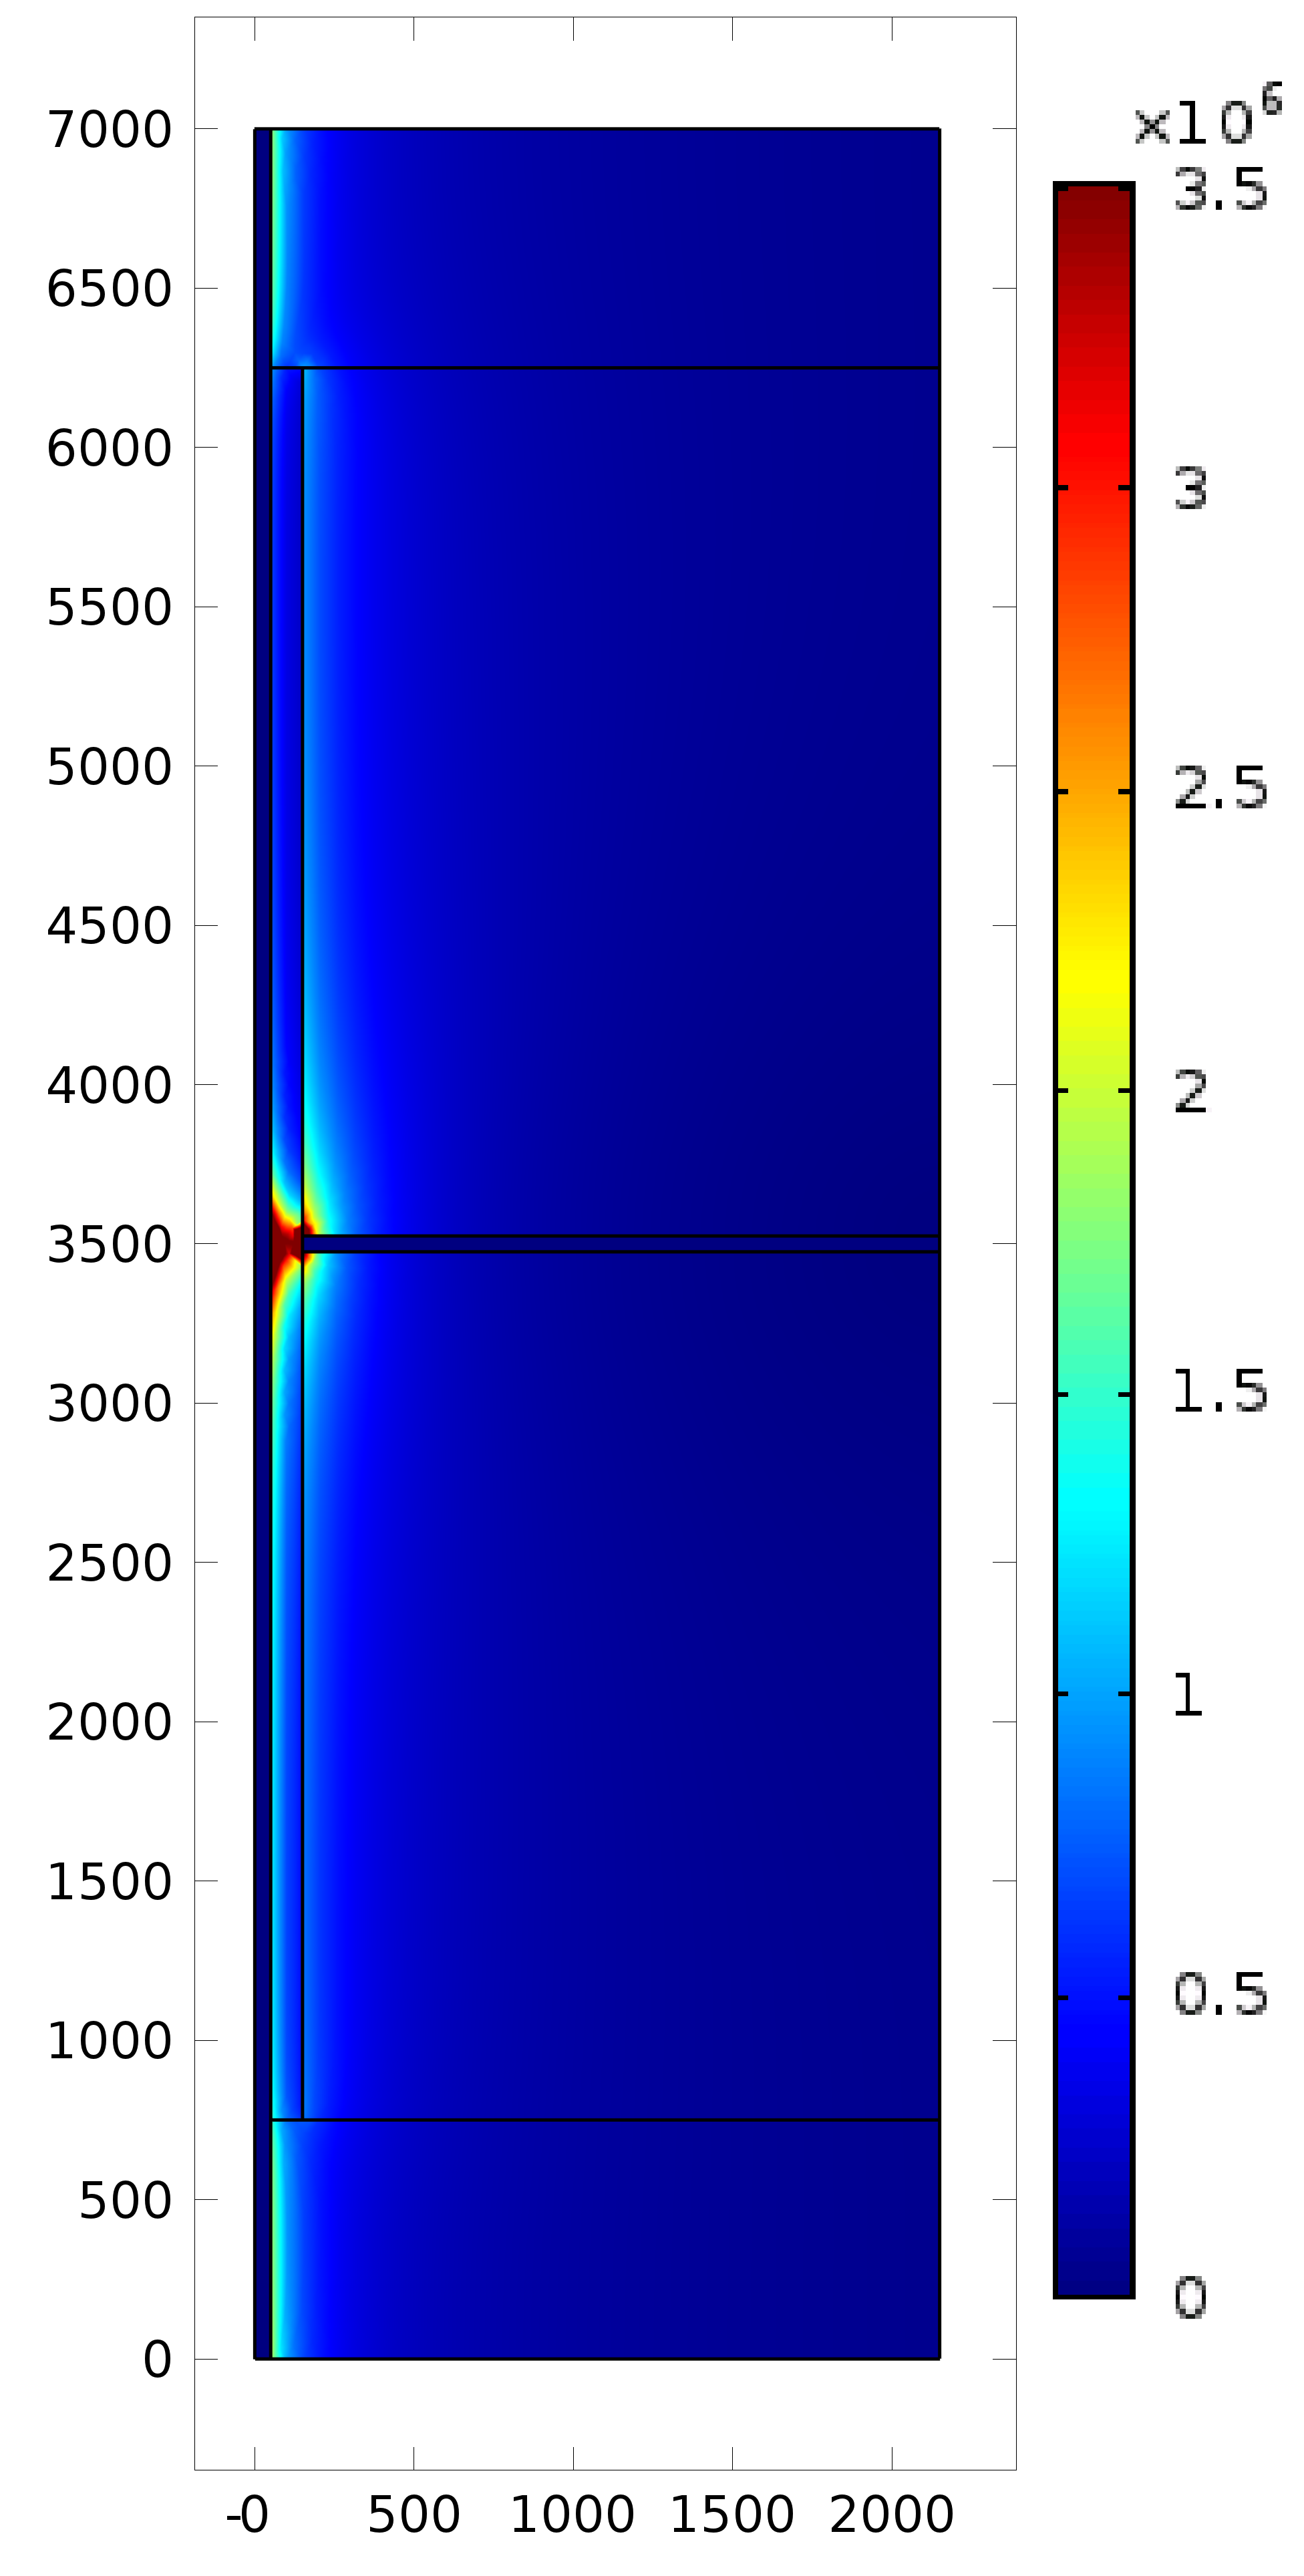
\includegraphics[width = 0.8\textwidth]{./Figures/Simulations/Edited_No_Foils_Large/Norm_E_Field.eps} 
\caption{Normal Electric Field (V/m) for Baseline Model}
\label{Figure:No_Foil_Large_Field}
\end{figure}

The model is made up with a very large geometry. 
The air and oil extends radially 2m from the end of the bushing and 1m in the axial direction.
This is to understand the anticipated area of interest in the model.
By considering figure \ref{Figure:No_Foil_Large_Field} it is clear that there is very little happening further than 500mm radially from the bushing surface and there is very little of interest further than 200mm in the radial direction.
Therefore all further models will adhere to this geometry, ensuring that the area of interest is captured, while decreasing simulation times to a minimum.

\subsection{No Foils}
In order to illustrate the requirement for capacitive grading within AC bushings, a simulation of a bushing with no grading was conducted.
Figure \ref{Figure:No_Foil_Geom} shows the geometry and materials used for each section.
The conductor length is $6000mm$ and has a width of half the inner diameter, $50mm$. 
The paper impregnated with oil insulation is $5500mm$ long in order to accommodate the first foil length of $5000mm$ with sufficient clearance. 
The transformer wall is modelled as a $50mm$ high aluminium block that is $500mm$ wide, and is placed vertically in the middle of the design. The surrounding oil and air are $500mm$ wide at the centre of the bushing, and extend to the length of the conductor.
The paper impregnated with oil insulation is sloped to avoid sharp corners and high field strengths.
\begin{figure}[!h]
  \centering
    \includegraphics[width = \textwidth]{./Figures/Simulations/Edited_No_Foils_Final/Geometry.eps} 
	\caption{Geometry and Materials for No Foils Bushing}
\label{Figure:No_Foil_Geom}
\end{figure}


A very fine mesh was used in this model as shown in figure \ref{Figure:No_Foil_Mesh}. This allows for the maximum level of accuracy in the results produced, and is possible since the geometry of this model is not over-complex.
\begin{figure}[!h]
  \centering
    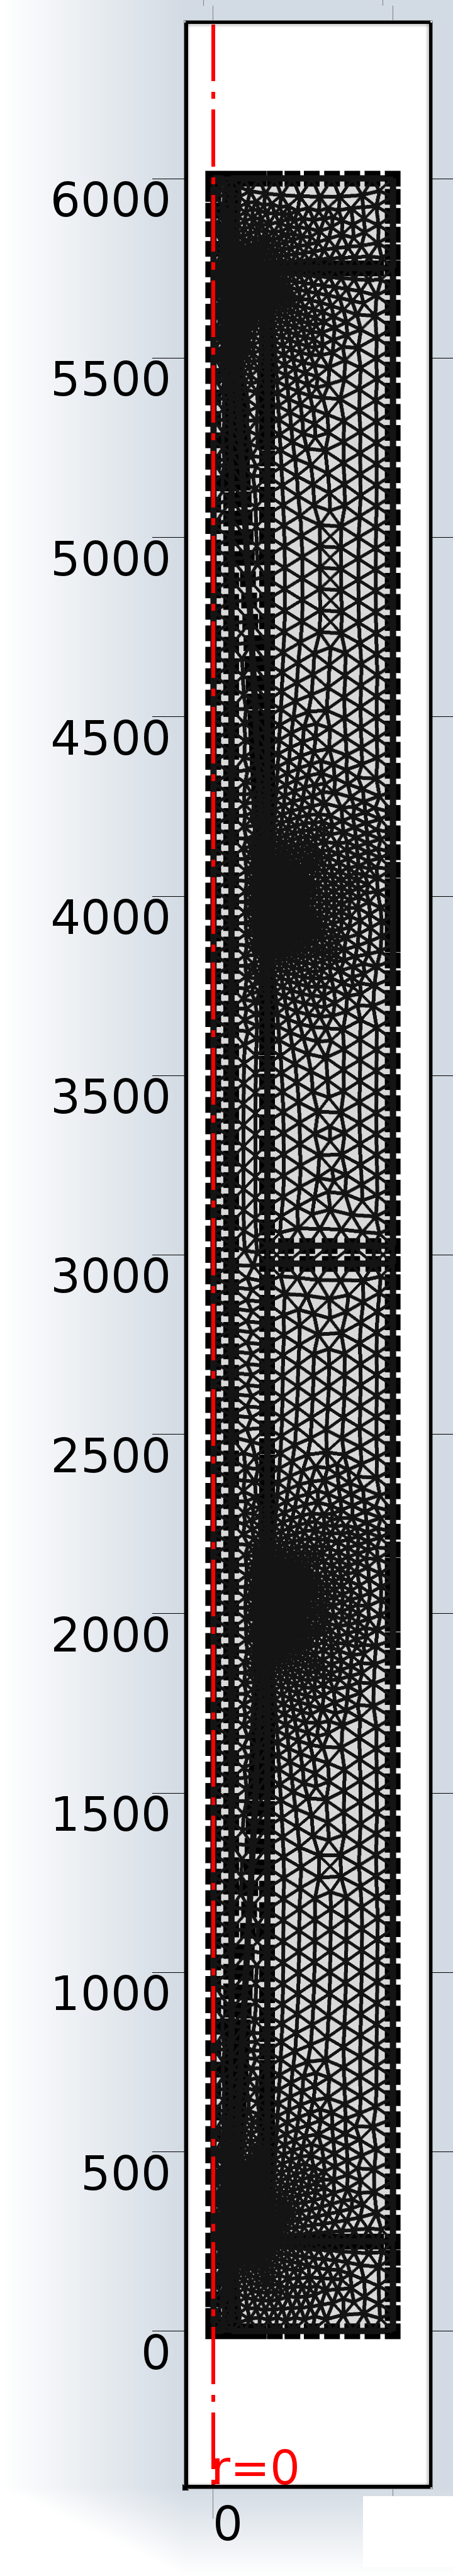
\includegraphics[width = \textwidth]{./Figures/Simulations/Edited_No_Foils_Final/Mesh.eps} 
	\caption{Extra Fine Mesh for No Foils Bushing}
\label{Figure:No_Foil_Mesh}
\end{figure}


\begin{figure}[!h]
  \centering
    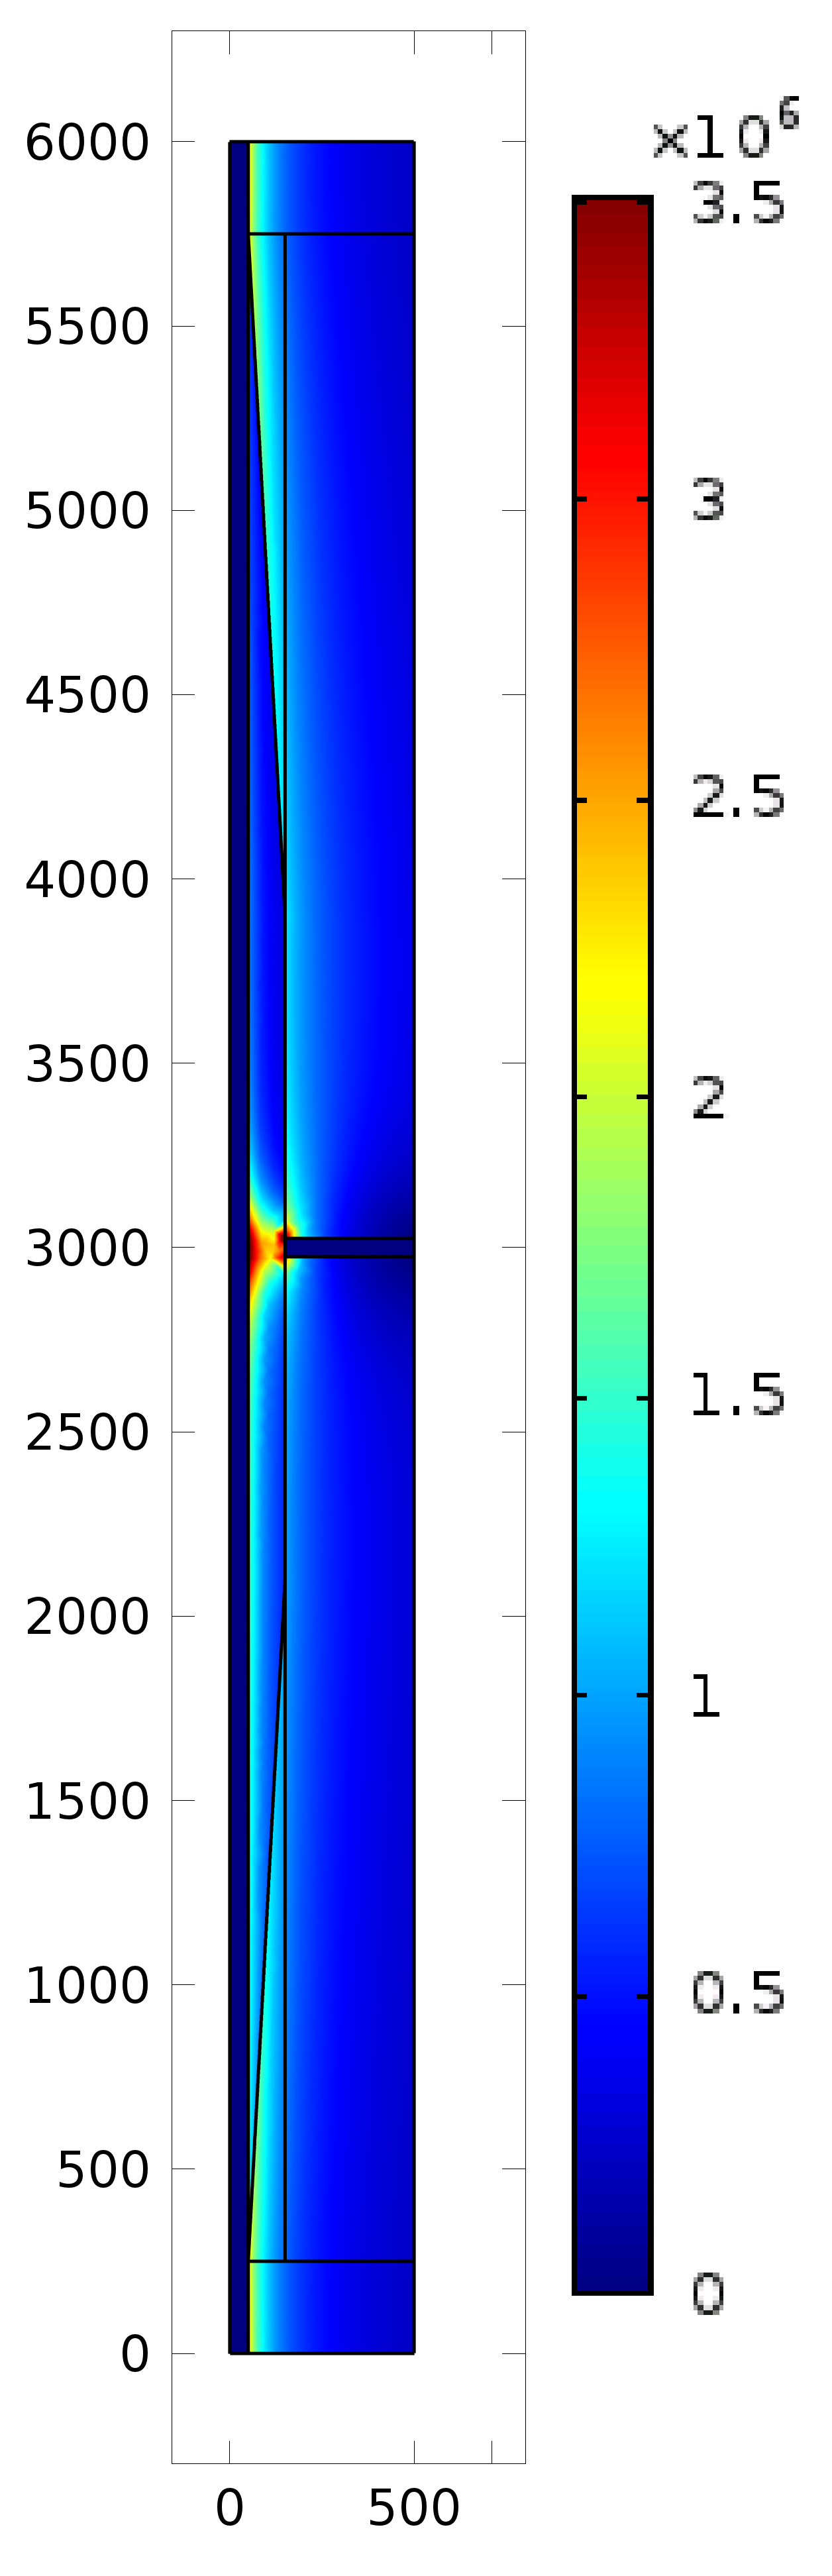
\includegraphics[width = \textwidth]{./Figures/Simulations/Edited_No_Foils_Final/E_Field_Norm.eps} 
	\caption{Normal Electric Field (V/m) for No Foils Bushing}
\label{Figure:No_Foil_Field}
\end{figure}


The motivation for capacitive grading is clear in figure \ref{Figure:No_Foil_Field}. 
The central area of stress is shown zoomed in figure \ref{figure:problemfield}.
The highest stress is shown at the corners of the transformer wall and in the plane between the transformer wall and the conductor.
This reaches field strengths greater than $3.5kV/mm$.
This simulation bears close resemblance to the theory explained in many texts and explained in figure \ref{figure:problem} in section \ref{s:method} of this report.
In order for this bushing to function within the design constraints, capacitive grading must be used.

\begin{figure}[!h]
   \centering
   \includegraphics[width = 0.5\textwidth]{./Figures/Simulations/Edited_No_Foils_Final/E_Field_Norm_Wall.eps}
   \caption{Area of very high electric stress}
   \label{figure:problemfield}
\end{figure}

\subsection{No Grading}
In order to rectify the high electric stress identified in the no foils model, isolated foils are introduced to capacitively grade the electric field.
To prove the requirement for grading the lengths or radial displacement of the foils, a simulation where the foils are maintained at the same length was performed.
The bushing has 21 foils spaced at an even radial spacing, but with no change in length of each foil.
Each foil is $1756mm$ in length, and is centred in the within the bushing. 

\begin{figure}[!h]
  \centering
    \includegraphics[width = \textwidth]{./Figures/Simulations/Edited_No_Grading_Final/Geometry.eps} 
	\caption{Geometry of the No Grading Model}
	\label{Figure:No_Grading_Geom}
\end{figure}

Producing a finite element mesh for this model caused issues with long computation time. 
Even using the coarsest default setting, the meshing time was of the order of days.
This is due to the difference in size of the aspects of the geometry.
The foils are just $0.1mm$ thick, which requires a very small set of triangles in order to mesh this area.
The other domains are up to $6000mm$ long, which is considerably larger and requires a different size of triangles.

In order to solves the issue, a set of meshing rules were produced.
Firstly, the mesh within the conductor and within the foils can be very coarse.
Within a conducting material, no electric field is expected, hence there is no reason to finely mesh that area.
Areas of interest or areas where the field changes rapidly need to have a very fine mesh to ensure the accuracy of the results is sufficient.
The meshing rules dictated a minimum number of points at the tip of each foil, and along the surface of the bushing.

\begin{figure}[!h]
  \centering
    \includegraphics[width = \textwidth]{./Figures/Simulations/Edited_No_Grading_Final/Mesh_wide.eps} 
	\caption{User defined meshing for no grading simulation - whole view}
\label{Figure:No_Grading_Mesh1}
\end{figure}

\begin{figure}[!h]
  \centering
    \includegraphics[width = 0.4\textwidth]{./Figures/Simulations/Edited_No_Grading_Final/Mesh_Close.eps} 
	\caption{User defined meshing for no grading simulation - foil tip view}
\label{Figure:No_Grading_Mesh2}
\end{figure}

Once the geometry has been meshed appropriately, the system can be solved to determine the electric field strength throughout the model, as shown in figure \ref{Figure:No_Grading_Field}.


\begin{figure}[!h]
  \centering
   \subfigure[Normal Electric Field (V/m) for the No-Grading Model]{
    \includegraphics[width = \textwidth]{./Figures/Simulations/Edited_No_Grading_Final/E_Field_Norm_Wide.eps} 
	%\caption{Normal Electric Field (V/m) for the No-Grading Model - Whole view}
	\label{Figure:No_Grading_Field_Wide}
   }\\

\subfigure[Normal Electric Field (V/m) in the Plane of the Transformer Wall]{
    \includegraphics[width = 0.45\textwidth]{./Figures/Simulations/Edited_No_Grading_Final/E_Field_Norm_Close_Mid.eps} 
	%\caption{Normal Electric Field (V/m) for the No-Grading Model}
	\label{Figure:No_Grading_Field_CloseMid}
   } \quad
\subfigure[Normal Electric Field (V/m) at the tips of the Foils]{
    \includegraphics[width = 0.45\textwidth]{./Figures/Simulations/Edited_No_Grading_Final/E_Field_Norm_Close_Tip.eps} 
	%\caption{Normal Electric Field (V/m) for the No-Grading Model}
	\label{Figure:No_Grading_Field_CloseTip}
   }
\caption{Examination of the Electric Field in the Non-Grading Model}
\label{Figure:No_Grading_Field}
\end{figure}

Simply adding foils into the bushing achieves nothing at all, and indicates the need for the grading methods used in the subsequent models.


\subsection{Radial Grading}
The geometry for the radial grading design is in figure \ref{Figure:Radial_Geom}. 
Each foil is an equal radial distance according to the radial grading method.
The lengths of each foil are determined from table \ref{table:radialvals}.
The remainder of the geometry is identical to the No Foils and No Grading models.
\begin{figure}[!h]
  \centering
    \includegraphics[width = \textwidth]{./Figures/Simulations/Edited_Radial_Final/Geometry.eps} 
	\caption{Geometry of the Radial Model}
	\label{Figure:Radial_Geom}
\end{figure}

As with the No Grading model, the geometry in this design is very complex with a variety of scales.
In order to reduce computation time but maintain a reasonable level of accuracy in areas of interest, the mesh was produced to the rules outlined for the No Grading model.
\begin{figure}[!h]
  \centering
    \includegraphics[width = \textwidth]{./Figures/Simulations/Edited_Radial_Final/Meshing.eps} 
	\caption{Meshing of the Radial Model}
	\label{Figure:Radial_Mesh_wide}
\end{figure}

\begin{figure}[!h]
  \centering
    \includegraphics[width = 0.7\textwidth]{./Figures/Simulations/Edited_Radial_Final/Mesh_Close.eps} 
	\caption{Meshing of the Radial Model Focused on a Foil Tip}
	\label{Figure:Radial_Mesh_close}
\end{figure}


\begin{figure}[!h]
  \centering
   %\subfigure[Normal Electric Field (V/m) for the No-Grading Model]{
    \includegraphics[width = \textwidth]{./Figures/Simulations/Edited_Radial_Final/E_Field_Norm_Wide.eps} 
	\caption{Normal Electric Field (V/m) for the Radial - Whole view}
	\label{Figure:Radial_Field_Wide}
   \end{figure}

\begin{figure}[!h]
  \centering
\subfigure[Normal Electric Field (V/m) in the Plane of the Transformer Wall]{
    \includegraphics[width = 0.35\textwidth]{./Figures/Simulations/Edited_Radial_Final/E_Field_Norm_Middle.eps} 
	%\caption{Normal Electric Field (V/m) for the No-Grading Model}
	\label{Figure:Radial_Field_CloseMid}
   } 
\subfigure[Normal Electric Field (V/m) at the tips of the Foils]{
    \includegraphics[width = 0.55\textwidth]{./Figures/Simulations/Edited_Radial_Final/E_Field_Norm_Tip.eps} 
	%\caption{Normal Electric Field (V/m) for the No-Grading Model}
	\label{Figure:Radial_Field_CloseTip}
   }
\caption{Examination of the Electric Field in the Radial Model}
\label{Figure:No_Grading_Field}
\end{figure}

The electric field in the system can now be analysed.
It can be seen in figure \ref{Figure:Radial_Field_CloseMid} that the field between the foils nearest the conductor is reduced to $3kV/mm$.
This is now evenly spread in the radial direction, as expected due to the radial grading of the electric field.

However, the electric field at the tips of the foils is not considered in the design method.
The field at the foil tips is largely due to the axial field strength, which is neglected during the radial grading design method.
It can be seen in figure \ref{Figure:Radial_Field_CloseTip} that the electric field at the tips of the foil is as large as $3.5kV/mm$.


\subsection{Axial Grading}
The asymmetric axial grading method results in an uneven geometry about the centre of the bushing.
This requires the paper insulation to take a different profile than the other models in order to adequately cover the foils, as shown in figure \ref{Figure:Axial_Geom}.
\begin{figure}[!h]
  \centering
    \includegraphics[width = \textwidth]{./Figures/Simulations/Edited_Axial_Final/Geometry.eps} 
	\caption{Geometry of the Axial Model}
	\label{Figure:Axial_Geom}
\end{figure}

\begin{figure}[!h]
  \centering
    \includegraphics[width = \textwidth]{./Figures/Simulations/Edited_Axial_Final/Meshing_Wide.eps} 
	\caption{Meshing of the Axial Model}
	\label{Figure:Axial_Mesh_wide}
\end{figure}

\begin{figure}[!h]
  \centering
    \includegraphics[width = 0.5\textwidth]{./Figures/Simulations/Edited_Axial_Final/Meshing_Tip.eps} 
	\caption{Meshing of the Axial Model Focused on a Foil Tip}
	\label{Figure:Axial_Mesh_close}
\end{figure}

\begin{figure}[!h]
  \centering
   %\subfigure[Normal Electric Field (V/m) for the No-Grading Model]{
    \includegraphics[width = \textwidth]{./Figures/Simulations/Edited_Axial_Final/E_Field_Norm_Wide.eps} 
	\caption{Normal Electric Field (V/m) for the Axial Model - Whole view}
	\label{Figure:Radial_Field_Wide}
   \end{figure}

\begin{figure}[!h]
  \centering
\subfigure[Normal Electric Field (V/m) in the Plane of the Transformer Wall]{
    \includegraphics[width = 0.45\textwidth]{./Figures/Simulations/Edited_Axial_Final/E_Field_Norm_Mid.eps} 
	%\caption{Normal Electric Field (V/m) for the No-Grading Model}
	\label{Figure:Radial_Field_CloseMid}
   } 
\subfigure[Normal Electric Field (V/m) at the tips of the Foils]{
    \includegraphics[width = 0.45\textwidth]{./Figures/Simulations/Edited_Axial_Final/E_Field_Norm_Tip.eps} 
	%\caption{Normal Electric Field (V/m) for the No-Grading Model}
	\label{Figure:Radial_Field_CloseTip}
   }
\caption{Examination of the Electric Field in the Axial Model}
\label{Figure:No_Grading_Field}
\end{figure}

\clearpage 

%\subsection{No Grading}
%As a baseline for comparison, a bushing with no foils has been constructed and simulated.
%The geometry of the model was built as in figure \ref{figure:Geom:Nograde}.
%The system is an axialsymmetric 2D model, which takes the central vertical point $r=0$ as the centre of a cylinder.
%\begin{figure}[!h]
%   \centering
%   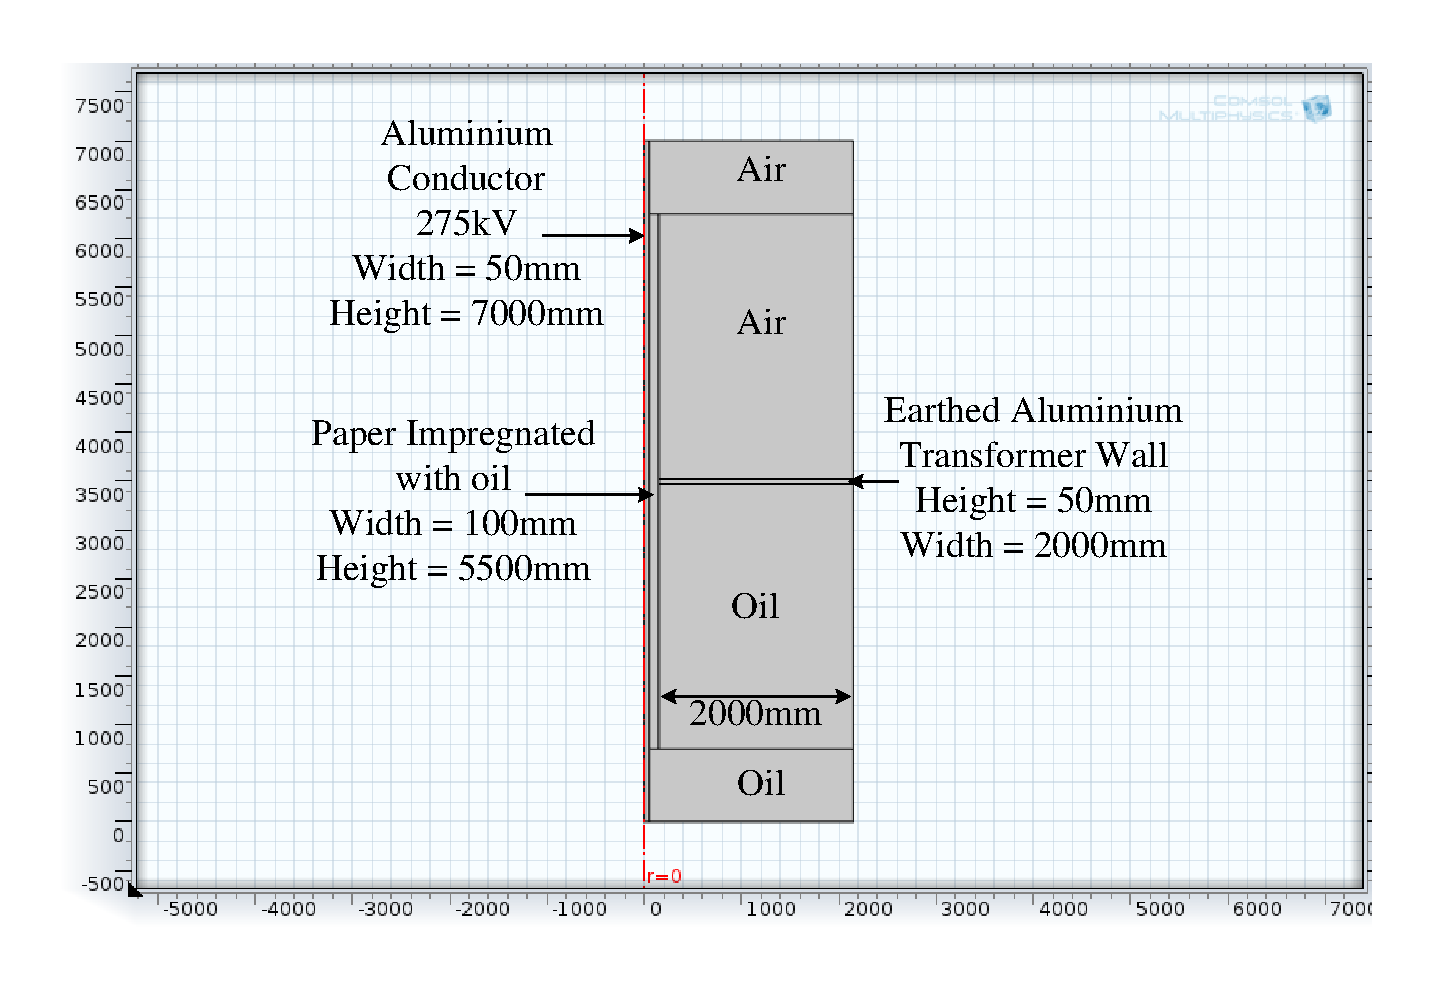
\includegraphics[width = 0.8\textwidth]{NoGradingBlock.pdf}
%   \caption{COMSOL Geometry Annotated with Materials - No Grading}
%   \label{figure:Geom:Nograde}
%\end{figure}
%
%Once the geometry of the model is defined, a finite element mesh can be created as shown in figure \ref{figure:Mesh:Nograde}.
%This model is fairly simple, hence a very fine graded mesh was used improving the accuracy of results.
%\begin{figure}[!h]
%   \centering
%   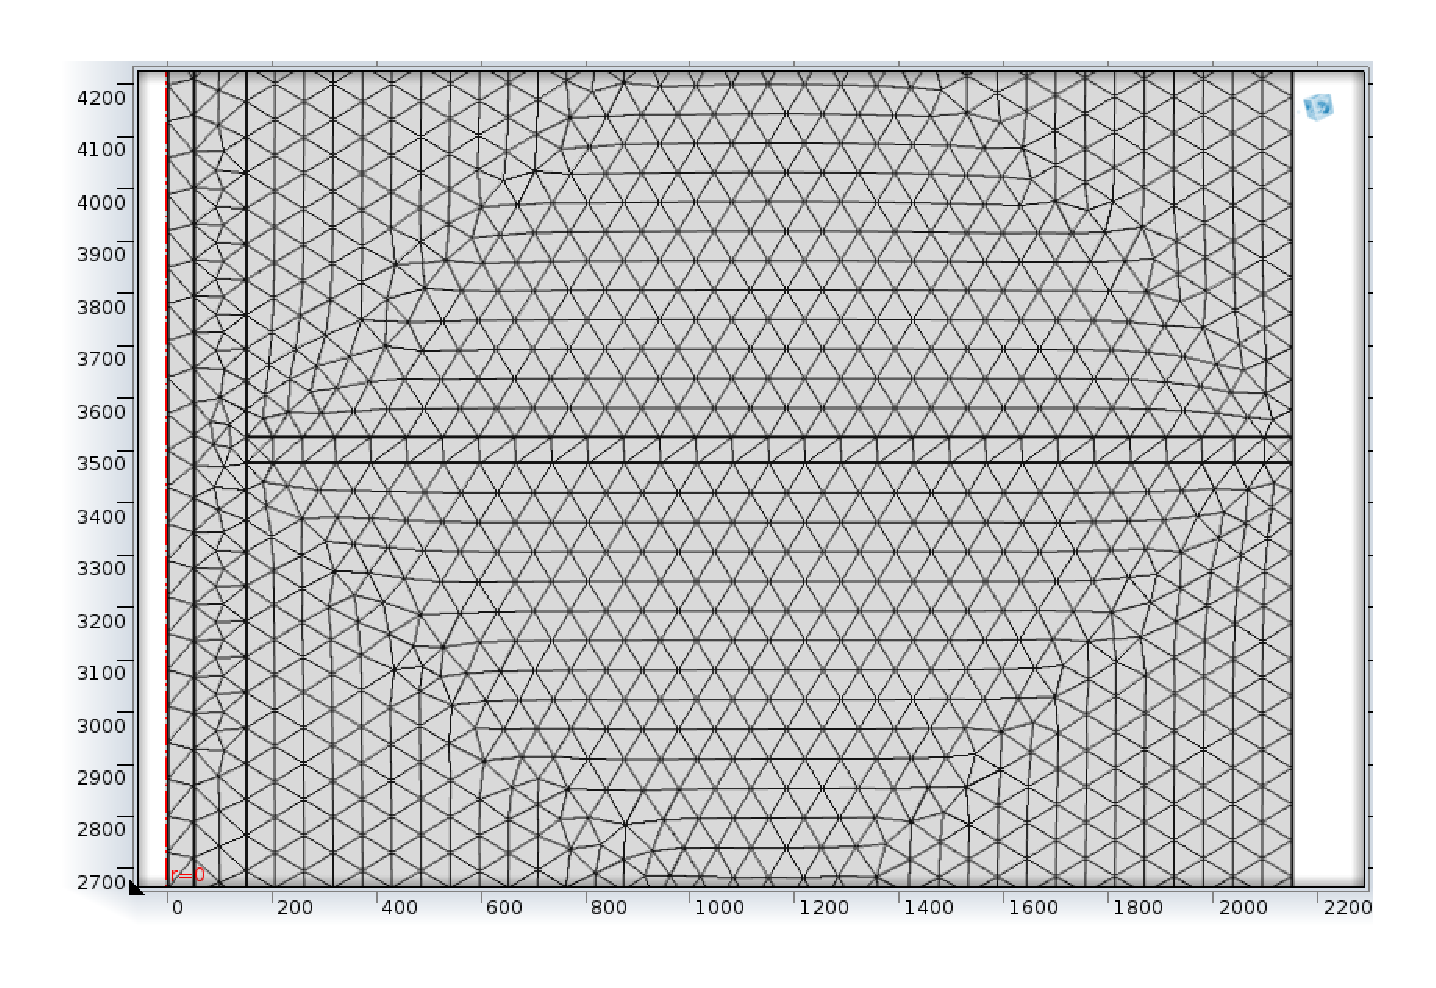
\includegraphics[width = 0.8\textwidth]{NoGradingMesh.pdf}
%   \caption{COMSOL Mesh - No Grading}
%   \label{figure:Mesh:Nograde}
%\end{figure}
%
%The next stage is to define the relative permittivity of each of the materials used for each sub section of the geometry.
%The initial conditions must then be set, with the conductor set to 275kV, and the transformer wall and all outer boundaries earthed.
%All other boundaries are assumed to be continuity boundaries.
%
%The model can then be solved to give the electric field distribution
%\inote{TS - Report done up to here 03/03/2014}
.
%\begin{figure}[!h]
%   \centering
%   \includegraphics[width = 0.8\textwidth]{WideNoGrading.png}
%\end{figure}
%
%\begin{figure}[!h]
%   \centering
%   \includegraphics[width = 0.8\textwidth]{CloseNoGrading.png}
%\end{figure}
%
%\begin{figure}[!h]
%   \centering
%   \includegraphics[width = 0.8\textwidth]{SurfaceGraded21.png}
%\end{figure}
%
%\begin{figure}[!h]
%   \centering
%   \includegraphics[width = 0.8\textwidth]{WideGraded21.png}
%\end{figure}
%
%\begin{figure}[!h]
%   \centering
%   \includegraphics[width = 0.8\textwidth]{CloseGraded21.png}
%\end{figure}
%
%\begin{figure}[!h]
%   \centering
%   \includegraphics[width = 0.8\textwidth]{SurfaceGradedCloseish21.png}
%\end{figure}
%  Discussion.tex
% !TeX spellcheck = en_GB
% !TeX root = ReportMain.tex

\section{Discussion} \label{s:Discussion}
As has been outlined in this report so far, there are problems inherent within bushing design and multiple solutions to these problems. A full discussion and comparison will be made to determine the most accurate and reliable model for HV bushing design. Additionally, reasoning and justification for the incremental changes will outline the development of bushing and possible further improvements that could be made in design.
%BH
\subsection{Success Criteria}
In section 2 four criteria were mentioned to determine the efficacy of the design: general/intrinsic breakdown defined by the radial field, surface discharge defined by the axial field, partial discharge within the material defined by areas of high tangential field and corona discharge within air. 

Regarding general breakdown it is the largest breakdown strength of the model and so the least likely to fail. High Voltage Engineering Fundamentals has it defined as well in excess of  1MV/cm \cite{kuffel2000high}. The area of interest for this intrinsic breakdown is the line from the conductor straight to the flange, and a measurement of radial electric field.

Surface discharge is not as readily defined for typical graded designs, however a comparison can be made from shedding specifications. Shedding increases the effective creepage length of the bushing by a factor of 4 and for a typical design 40mm/kV is given as the required length for the operational voltage \cite{HVEngandTesting}.

Fortunately and reasonably given its significance, partial discharge inception voltage is well defined for all types of insulation material. For resin-impregnated paper the value is 36kV/cm and for oil-impregnated paper the value is 45kV/cm, justifying the more common use of OIP \cite{HVEngandTesting}. Due to its nature, a simple investigation of trends is not sufficient to estimate areas of possible PD origins and areas of interest must be found and tested against the inception voltage. They are typically located at the edges of foils or near the conductor itself.

Corona discharge can occur in both air and oil, however, since the inception voltage is much lower for air and the effects of weather and pollution affect the air side of the bushing much greater it is of higher importance. For the discussion, it will be studied as a subsection of surface discharge.  

\subsection{No Foils}
%BH
%fig 6.7
Nowadays, solid bushing is only used for voltages below 25kV. This is due to a combination of all factors as shown in the previous figure 6.7. When simulated with a conductor ten times its rated voltage its flaws are clear. As mentioned previously, the primary criteria to solve are high electric fields inducing partial discharges and large axial fields causing flashover. 

\begin{figure}[!h]
  \centering
    \includegraphics[width = 0.8\textwidth]{../Simulations/DataSets/No_Foil_Fail.eps} 
\caption{The No Foils Model Fails PD Criteria}
\label{Figure:NoFoilsFail}
\end{figure}

This is best illustrated with figure 7.1, not only are the fields present at the interface to the flange well in excess of the PD inception voltage, the location of these high electric fields also mean flashover is a serious risk due to the lack of shaping of the axial electric field distribution. A result of such localised electric stress is that because the field is greater than the PD inception voltage the voids will generate exponentially more discharges, leading to faster ageing and a much higher chance of breakdown. The solution, assuming keeping voltage constant, would be to increase the bushing height and width. 
\subsection{No Grading}
%BH
%fig 6.11b, 6.11c
%same graph as 7.1 but for no grading
%done but need to make .fig into pdf then add to latex (help needed)
The proposal to study a model of condenser bushing without any thought to grading exposes the fundamentals to grading design. Figure 7.2 shows that, for the most part the electric field is below the PD inception voltage, at least at the central interface. However looking at figures 6.11b and 6.11c show that the foil placement did not effectively shape the field at the bushing interface at the tips.  Beyond analysing the concentrations of electric field it is important to note that the distribution is non-linear; in comparison to the ideal goal of a linear drop of field across the capacitors \citep{kuffel2000high}. The placement of the outermost foil serves as a location of high field density and although located far from the flange itself it would likely be a source of both PDs and corona discharges. 
% want a plot of the tips?

\subsection{Comparison of Axial and Radial Grading Solutions}
The design of both types of capacitive grading method were discussed in the previous sections. The difference in performance of the types in general is the radial grading will improve the intensity of the radial electric field and the axial grading will improve the intensity of the axial electric field. By improvement of intensity of electric field, this means the electric field according to the type of grading method is evenly distributed in a particular direction. Choosing the right design for different application is essential as this will reduce the chances of various types of electrical breakdown and hence the bushing design would be more durable.

There are two components of electric field cause different problems. The radial electric field is mainly responsible to the breakdown of insulating material, for example, electrical breakdown between foils. On the other hand, the axial electric field is mainly responsible to the surface discharges along the boundary of the insulation, for example, corona discharge to the surrounding.

\subsubsection{Radial Electric Field}
The maximum intensity of the radial electric field for the radial design is expected to be lower than the maximum of the axial design. This means the radial grading design would perform better to suppress the intensity of radial electric field. The radial electric field across the radial direction of both axial and radial grading designs are shown in figure \ref{figure:rfield}.

\begin{figure}[!h]
\centering
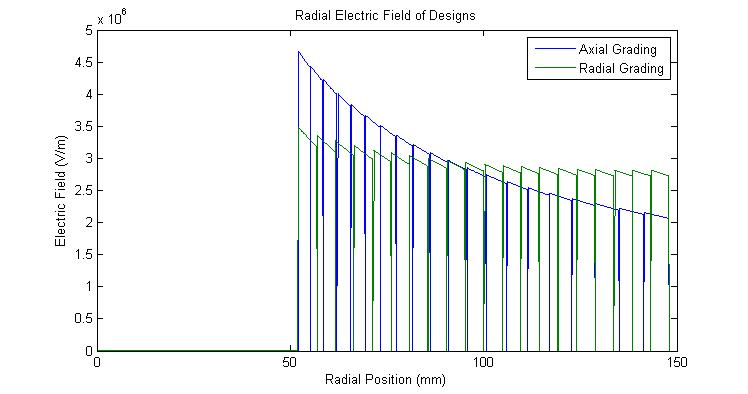
\includegraphics[width = \textwidth]{R-field.jpg}
\caption{Radial electric field across the mid-point of the two designs of bushing.}
\label{figure:rfield}
\end{figure}

The result clearly shows the peak value of electric field for the axial design ($\approx 4.5 \times 10^3 kVm^{-1}$) is greater than the peak value of electric field for the radial design ($\approx 3.5 \times 10^3 kVm^{-1}$). Also, from the figure \ref{figure:rfield}, the radial electric field of the radial grading design is more evenly distributed. This is the effect of grading, hence similar effect should be seen in the axial electric for axial grading design. The electric field distribution across any perpendicular cut lines to the foils would result in almost identical results, because the foils behave similar to capacitors in series. Electric field being constant across a capacitor and this is true across any two neighbouring foils.

\subsubsection{Axial Electric Field}
The axial component of electric field is responsible for the surface discharges along the surface of the bushing design. Axial component of the field contributes to these surfaces, because the axial electric field at the edges of the foil are the most intense. Figure \ref{figure:afield} shows the magnitude of electric field at each foil edge. 

\begin{figure}[!h]
\centering
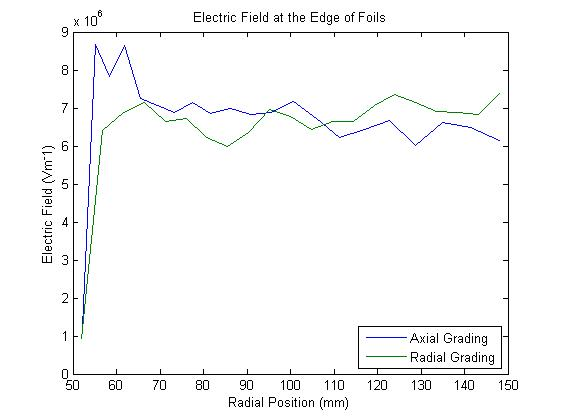
\includegraphics[width = \textwidth]{A-field.jpg}
\caption{Electric field at the edge of each foil.}
\label{figure:afield}
\end{figure}
%this graph is a mess, I took very long time to convince myself to put this on here. This is the best I can do at the moment

The result shows the radial design has a lower peak value of electric field at these edges of foil. However, this is not an expected result, because axial grading in theory shapes the surface of the insulation better to avoid intensifying of electric field at these edges. Also, a clearer maximum peak of electric field at should be seen at the outermost foil of the radial graded design due to the sharp turn in the shape of the bushing design. Although the result shows a maximum peak at the last outermost foil, it is not significant and it is below the maximum value of electric field for the axial graded design.

\subsubsection{Surface Flashover}
%talk about the addition of shedding in completeness. Limitations of current model without shedding -> primarily some extra shaping of fields. The effect of grounding the outermost capacitor.
%===============================================
Surface flashover is the partial discharge along the surface of the insulation, this is cause by a intense electric field. The parameter which takes into account of surface flashover is the creepage distance as mention previously. The typical value for calculating the creepage distance is 35mm/kV %need a reference for this prob%
and for more polluted environment, a higher value of creepage distance might be considered.

In bushing designs, the creepage distance is increased by the addition of a shed around the bushing. These shed designs increase the creepage distance of insulation designs by increasing the surface length.  Designs of shed can have varying ratios between creepage distance to axial length \cite{shed}, designs for more polluted environment have bigger ratios.

According to the typical value to calculate the creepage distance, for a 275kV design, the creepage distance required is 9625mm. Where the designs of bushing in this report has axial length of approximately 3m, the ratio of minimum nominal creepage distance to axial length required is 3.2:1.

These shed provides a greater creepage distance to reduce the chance of surface flashover, however, they have little affect on the electric field of the bushing. Hence, addition of shed does not reduce corona discharge. 

\subsection{Choice of Designing Method}

\section{Conclusions}
Conclusions.

%regarding area of interest of tips of foils a suggestion in (Graham?) was to line the capacitors with semiconductor material to more evenly spread out the field distribution.

%% ----------------------------------------------------------------
%You probably found all the files from \cite{Gunn:2001:pdflatex}.
%\tref{Table:tabex} illustrates the results of my work~\citep{Gunn:2011:updated2}.
%\begin{table}[!htb]
%  \centering
%  \begin{tabular}{cc}
%  \toprule
%  \textbf{Training Error} & \textbf{Testing Error}\\
%  \midrule
%  0 & $\infty$\\
%  \bottomrule
%  \end{tabular}
%  \caption{The Results}
%  \label{Table:tabex}
%\end{table}
%
%\fref{Figure:figex} shows why this is the case.
%\begin{figure}[!htb]
%  \centering
%  \includegraphics[width=8cm]{figure}
%  \caption{A colourful picture.}
%  \label{Figure:figex}
%\end{figure}
%
%This page shows you a subfigure example in \fref{Figure:figsubex}.
%\begin{figure}[!htb]
%  \centering
%  \subfigure[The left caption]{
%    \includegraphics[width=4.2cm]{figure}
%    \label{Figure:figsubex:left}
%  }
%  \subfigure[The right caption]{
%    \includegraphics[width=4.2cm]{figure}
%    \label{Figure:figsubex:right}
%  }
%  \caption{A doubly colourful picture.}
%  \label{Figure:figsubex}
%\end{figure}
%

\backmatter
\bibliographystyle{unsrt}
\bibliography{ECS}
\appendix
%\include{appendix_stuff}
\end{document}
%% ----------------------------------------------------------------
